% Options for packages loaded elsewhere
\PassOptionsToPackage{unicode}{hyperref}
\PassOptionsToPackage{hyphens}{url}
%
\documentclass[
]{article}
\usepackage{amsmath,amssymb}
\usepackage{lmodern}
\usepackage{iftex}
\ifPDFTeX
  \usepackage[T1]{fontenc}
  \usepackage[utf8]{inputenc}
  \usepackage{textcomp} % provide euro and other symbols
\else % if luatex or xetex
  \usepackage{unicode-math}
  \defaultfontfeatures{Scale=MatchLowercase}
  \defaultfontfeatures[\rmfamily]{Ligatures=TeX,Scale=1}
\fi
% Use upquote if available, for straight quotes in verbatim environments
\IfFileExists{upquote.sty}{\usepackage{upquote}}{}
\IfFileExists{microtype.sty}{% use microtype if available
  \usepackage[]{microtype}
  \UseMicrotypeSet[protrusion]{basicmath} % disable protrusion for tt fonts
}{}
\makeatletter
\@ifundefined{KOMAClassName}{% if non-KOMA class
  \IfFileExists{parskip.sty}{%
    \usepackage{parskip}
  }{% else
    \setlength{\parindent}{0pt}
    \setlength{\parskip}{6pt plus 2pt minus 1pt}}
}{% if KOMA class
  \KOMAoptions{parskip=half}}
\makeatother
\usepackage{xcolor}
\usepackage[margin=1in]{geometry}
\usepackage{graphicx}
\makeatletter
\def\maxwidth{\ifdim\Gin@nat@width>\linewidth\linewidth\else\Gin@nat@width\fi}
\def\maxheight{\ifdim\Gin@nat@height>\textheight\textheight\else\Gin@nat@height\fi}
\makeatother
% Scale images if necessary, so that they will not overflow the page
% margins by default, and it is still possible to overwrite the defaults
% using explicit options in \includegraphics[width, height, ...]{}
\setkeys{Gin}{width=\maxwidth,height=\maxheight,keepaspectratio}
% Set default figure placement to htbp
\makeatletter
\def\fps@figure{htbp}
\makeatother
\setlength{\emergencystretch}{3em} % prevent overfull lines
\providecommand{\tightlist}{%
  \setlength{\itemsep}{0pt}\setlength{\parskip}{0pt}}
\setcounter{secnumdepth}{-\maxdimen} % remove section numbering
\newlength{\cslhangindent}
\setlength{\cslhangindent}{1.5em}
\newlength{\csllabelwidth}
\setlength{\csllabelwidth}{3em}
\newlength{\cslentryspacingunit} % times entry-spacing
\setlength{\cslentryspacingunit}{\parskip}
\newenvironment{CSLReferences}[2] % #1 hanging-ident, #2 entry spacing
 {% don't indent paragraphs
  \setlength{\parindent}{0pt}
  % turn on hanging indent if param 1 is 1
  \ifodd #1
  \let\oldpar\par
  \def\par{\hangindent=\cslhangindent\oldpar}
  \fi
  % set entry spacing
  \setlength{\parskip}{#2\cslentryspacingunit}
 }%
 {}
\usepackage{calc}
\newcommand{\CSLBlock}[1]{#1\hfill\break}
\newcommand{\CSLLeftMargin}[1]{\parbox[t]{\csllabelwidth}{#1}}
\newcommand{\CSLRightInline}[1]{\parbox[t]{\linewidth - \csllabelwidth}{#1}\break}
\newcommand{\CSLIndent}[1]{\hspace{\cslhangindent}#1}
\usepackage{lineno}
\linenumbers
\usepackage{setspace}\doublespacing
\usepackage{gensymb}
\usepackage{float}
\ifLuaTeX
  \usepackage{selnolig}  % disable illegal ligatures
\fi
\IfFileExists{bookmark.sty}{\usepackage{bookmark}}{\usepackage{hyperref}}
\IfFileExists{xurl.sty}{\usepackage{xurl}}{} % add URL line breaks if available
\urlstyle{same} % disable monospaced font for URLs
\hypersetup{
  pdftitle={Quantifying Impacts of an Environmental Intervention Using Environmental DNA},
  pdfauthor={Elizabeth Andruszkiewicz Allan,; Ryan P. Kelly,; Erin D'Agnese,; Maya Garber-Yonts,; Megan Shaffer,; Zachary Gold,; Andrew O. Shelton},
  hidelinks,
  pdfcreator={LaTeX via pandoc}}

\title{Quantifying Impacts of an Environmental Intervention Using
Environmental DNA}
\author{Elizabeth Andruszkiewicz Allan, \and Ryan P. Kelly, \and Erin
D'Agnese, \and Maya Garber-Yonts, \and Megan Shaffer, \and Zachary
Gold, \and Andrew O. Shelton}
\date{2022}

\begin{document}
\maketitle

{[}Draft for \emph{Ecological Applications}, Fall 2022{]}

\hypertarget{abstract}{%
\subsection{Abstract}\label{abstract}}

Environmental laws around the world require some version of an
environmental impact assessment surrounding construction projects and
other discrete instances of human development. Information requirements
for these assessments vary by jurisdiction, but nearly all require an
analysis of the living elements of affected ecosystems. Because it is
possible to sample and amplify the genetic material of many species
present in those environments, amplicon-sequencing --- also called
metabarcoding or environmental DNA (eDNA) analysis --- is a tractable,
powerful, and increasingly common way of doing environmental impact
analysis for development projects. Here, we analyze a 12-month
time-series of water samples taken before, during, and after a
construction project in a salmonid-bearing freshwater stream. We use an
asymmetrical Before-After-Control-Intervention (BACI) design with
multiple control streams to develop a robust background expectation
against which to evaluate the impact of this discrete human intervention
in the treatment stream. We generate calibrated, quantitative
metabarcoding data from amplifying a fragment of the 12s mtDNA gene and
complementary qPCR data to yield multi-species estimates of absolute
eDNA abundance across time, creeks, and sampling stations. We then use a
hierarchical Bayesian time-series model to reveal patterns of eDNA
concentrations over time, and to estimate the effects of the culvert
removal on salmonids in the treatment creek. We focus our analysis on
four common salmonid species in the data: cutthroat trout
(\emph{Oncorhynchus clarkii}), coho trout (\emph{O. kisutch}), rainbow
trout (\emph{O. mykiss}), and sockeye salmon (\emph{O. nerka}). After
accounting for temporal variability common to the sampled creeks, we
find only transient effects on these species during the several months
after construction. In the context of billions of dollars of
court-mandated road culvert replacements taking place in Washington
State, USA, our results suggest that culvert replacement can be
conducted with only minimal impact to key species of management concern.
More broadly, we demonstrate a rigorous, quantitative method for
environmental impact reporting using eDNA that is widely applicable in
environments worldwide.

\hypertarget{introduction}{%
\subsection{Introduction}\label{introduction}}

At present, it is difficult or impossible to measure the environmental
impacts of discrete human activities, despite such assessment often
being required by law. Within the United States, both state and federal
laws often require a form of environmental-impact assessment for medium-
to large-scale projects (i.e., those that might have a significant
impact on the environment) (Morgan, 2012). Outside the US, many nations
have their own versions of these same laws. Specifically when measuring
impacts on aquatic ecosystems, assessments generally continue to rely on
literature reviews or field measurements of a few key species, selected
beforehand (Rubin et al., 2017). These traditional methods are often
expensive, rely on just a few species, and are extremely limited in
spatial and temporal coverage (Martin et al., 2012). Moreover, they
often lack pre- or post-project monitoring, or sufficient post-project
sampling, given that the goals of a development project normally focus
on construction itself and funding is often extremely limited. For
example, a recent literature review of stream restoration projects cites
that more than half of projects (62\%) had no pre-project monitoring and
only sampled once per year (Rubin et al., 2017).

All methods of environmental sampling are biased, in the sense that they
capture a selective portion of the biodiversity present (Rubin et al.,
2017). Net samples for fish, for example, fail to capture species too
small or too large to be caught in the net; bacterial cultures capture
only those species that can be cultured on available media, and so
forth. Despite the pleasing simplicity of the idea, there is no one way
to survey the world and just ``see what is there.'' Environmental DNA,
however, comes as close to this goal as any method yet developed: a
sample of water, soil, or even air, contains the genetic traces of many
thousands of species, from microbes to whales. Sequencing environmental
DNA (eDNA) is means of surveying many species in a consistent and
scaleable way (Taberlet et al., 2012; Thomsen and Willerslev, 2015).
Sampling water to collect eDNA before, during, and after a development
project would be a new and powerful way of assessing that project's
impacts on the local biological communities, and conceivably could
become the standard way to do such impact assessment (Hinz et al.,
2022). Environmental assessments have begun to make use of eDNA for such
work around the world (Duda et al., 2021; Klein et al., 2022; Maasri et
al., 2022; Moss et al., 2022; Muha et al., 2017), but are not yet common
practice.

Surveying the natural world by amplifying and sequencing DNA from
environmental sources such as water, air, or soil has long been
commonplace in microbial ecology (Ogram et al., 1987; Rondon et al.,
2000; Turnbaugh et al., 2007), but has recently become popular for
characterizing ecological communities of eukaryotes (De Vargas et al.,
2015; Kelly et al., 2014; Port et al., 2015; Stat et al., 2017; Taberlet
et al., 2012; Valentini et al., 2016). Because the source of samples is
the environment itself (e.g., water) rather than specific target
organisms, the data resulting from such studies have become known as
environmental DNA (eDNA); the ultimate source of genetic material in the
environment may be living or waste cells or extracellular DNA (Taberlet
et al., 2012). Techniques that take advantage of such data may include
non-PCR-based methods such as hybridization, but generally include an
amplification step such as quantitative PCR, digital or digital-droplet
PCR, or traditional PCR from mixed templates followed by high-throughput
sequencing (Ruppert et al., 2019). This last technique is known as
metabarcoding, eDNA amplicon-sequencing, or more generally, marker-gene
analysis.

In a metabarcoding approach, broad-spectrum PCR primers capture many
taxa across a very wide diversity of the tree of the life (e.g., Leray
et al. (2013)), but nevertheless the absence of a taxon from a sequenced
sample does not indicate the absence of that taxon from the environment
(Buxton et al., 2021; Kelly et al., 2019; Shelton et al., 2016).
Instead, the unsampled species simply may not have been susceptible to
that set of PCR primers, and so failed to amplify. The result is often a
dataset that represents hundreds or thousands of taxa, but these taxa
are a fraction of a larger (and perhaps taxonomically broad) pool of
species present. Using multiple, independent primer sets increases
taxonomic scope by drawing from overlapping pools of taxa (Kelly et al.,
2017), maximizing the likelihood of detecting any given taxon present.
In virtually all comparisons, metabarcoding recovers far more taxa from
an area than any other sampling method (Kelly et al., 2017; Port et al.,
2015; Seymour et al., 2021).

However, we expect results from metabarcoding to differ dramatically
from non-PCR based sampling methods due to the fundamental differences
in sampling for genetic waste as opposed to whole organisms. Futhermore,
eDNA analyses rely on several laboratory processes, including PCR
amplification, all of which contribute to complicating the
interpretation of results (see Shelton et al. (2016) and Kelly et al.
(2019) for more information). Specifically, the PCR amplification
process is an exponential process for which the efficiency varies across
species. By understanding these process differences, we can correct for
taxon-specific biases in amplification efficiency to yield quantitative
estimates of the community composition prior to PCR (McLaren et al.,
2019; Shelton et al., 2022).

The resulting metabarcoding dataset is compositional, revealing the
proportions of each species' DNA present in each sample, but
importantly, contains no information about the absolute abundance of DNA
present. We can tie these proportional estimates to absolute abundances
using additional data such as a qPCR assay for one of the taxa present.
Thus, we can use qPCR and metabarcoding together to maximize the
information gleaned from the same samples by obtaining information about
many species through metabarcoding, and then grounding the compositional
dataset to quantifications provided from the results of a qPCR assay for
a single species that is also detected in the metabarcoding approach.
Together, we can use these data to assess changes in eDNA concentrations
of species over time, and due to environmental impacts such as replacing
a culvert under a road.

As a result of a federal court ruling (Martinez, 2013), Washington State
is under a court order to replace hundreds of culverts that allow water
to pass under roads and highways. The culverts that need to be replaced,
at present, collectively prevent or hinder anadromous salmon species
from using hundreds of miles of habitat, which in turn violates the
treaty rights of the region's indigenous tribes. Because replacing
culverts can require substantial intervention -- for example, diverting
the water from a creek segment and rebuilding the road with a redesigned
culvert -- they require environmental impact assessments. Furthermore,
because these replacements occur serially according to a schedule, they
present an attractive experimental design to use eDNA to assess
environmental impacts.

Here, we report the results of a yearlong eDNA sampling effort before,
during, and after a small construction project in our experimental
creek, assessing the impact of that project on the salmonid species
present. We do so using a combination of metabarcoding (12s mtDNA) and
qPCR to yield quantitative estimates of the concentrations of DNA
present at each time point, and we use parallel samples from an
additional four control creeks to develop a causal analysis of changes
in these concentrations. A clear opportunity for policy-relevant eDNA
work is in using its power to survey many species at a time to improve
the way we assess the impacts of human activities. We demonstrate the
utility of eDNA for such assessments.

\hypertarget{methods}{%
\subsection{Methods}\label{methods}}

We used an asymmetrical BACI (Before-After-Control-Impact) study design
to measure the environmental impact of a construction project replacing
the under-road culvert in the treatment creek using eDNA
(Benedetti-Cecchi, 2001; Underwood, 1994, 1992). We sampled four control
creeks in addition to the treatment creek (Figure \ref{fig:map}) at
monthly intervals, both upstream and downstream of each creek's culvert.
Because salmonids are the primary species of management concern in these
creeks, we focus the present analysis on the four salmonid species most
common in our data: \emph{Oncorhynchus clarkii} (cutthroat trout),
\emph{O. kisutch} (coho salmon), \emph{O. mykiss} (rainbow and steelhead
trout), and \emph{O. nerka} (sockeye and kokanee salmon). As further
described below, we surveyed the salmonid DNA present in each creek via
eDNA metabarcoding (targeting a region of the 12s mtDNA gene) and
complementary quantitative PCR (qPCR; targeting a region of the CytB
gene) for a reference species (\emph{O. clarkii}), which in combination
yielded quantitative estimates for each fish species throughout the
study area.

Construction to replace the culvert in our treatment creek occurred
midway through our year-long survey. We were then able to quantify the
effect of the culvert replacement itself -- controlling for temporal
trends, background environmental variability, and sampling variability
-- using a Bayesian time-series model to jointly model salmon eDNA
abundances across creeks, time points, sampling stations, and species.

\hypertarget{water-sampling}{%
\subsubsection{Water Sampling}\label{water-sampling}}

We collected water samples monthly between March 2021 and February 2022
in each of five salmonid-bearing creeks in northwest Washington State,
USA (Figure \ref{fig:map}). We sampled each stream above and below
under-road culverts, each of with a different degree of expected fish
passibilty as determined by the Washington Department of Transportation
(Supplemental Text 1) (Fish and Wildlife, 2019). The culvert in the
treatment creek (Padden) was suspected to be impassible and thus was
removed and replaced during the course of the study; two of the four
creeks had culverts allowing fish passibility (Portage and Squalicum),
and two had culverts blocking fish passage (Barnes and Chuckanut).

\begin{figure}
\centering
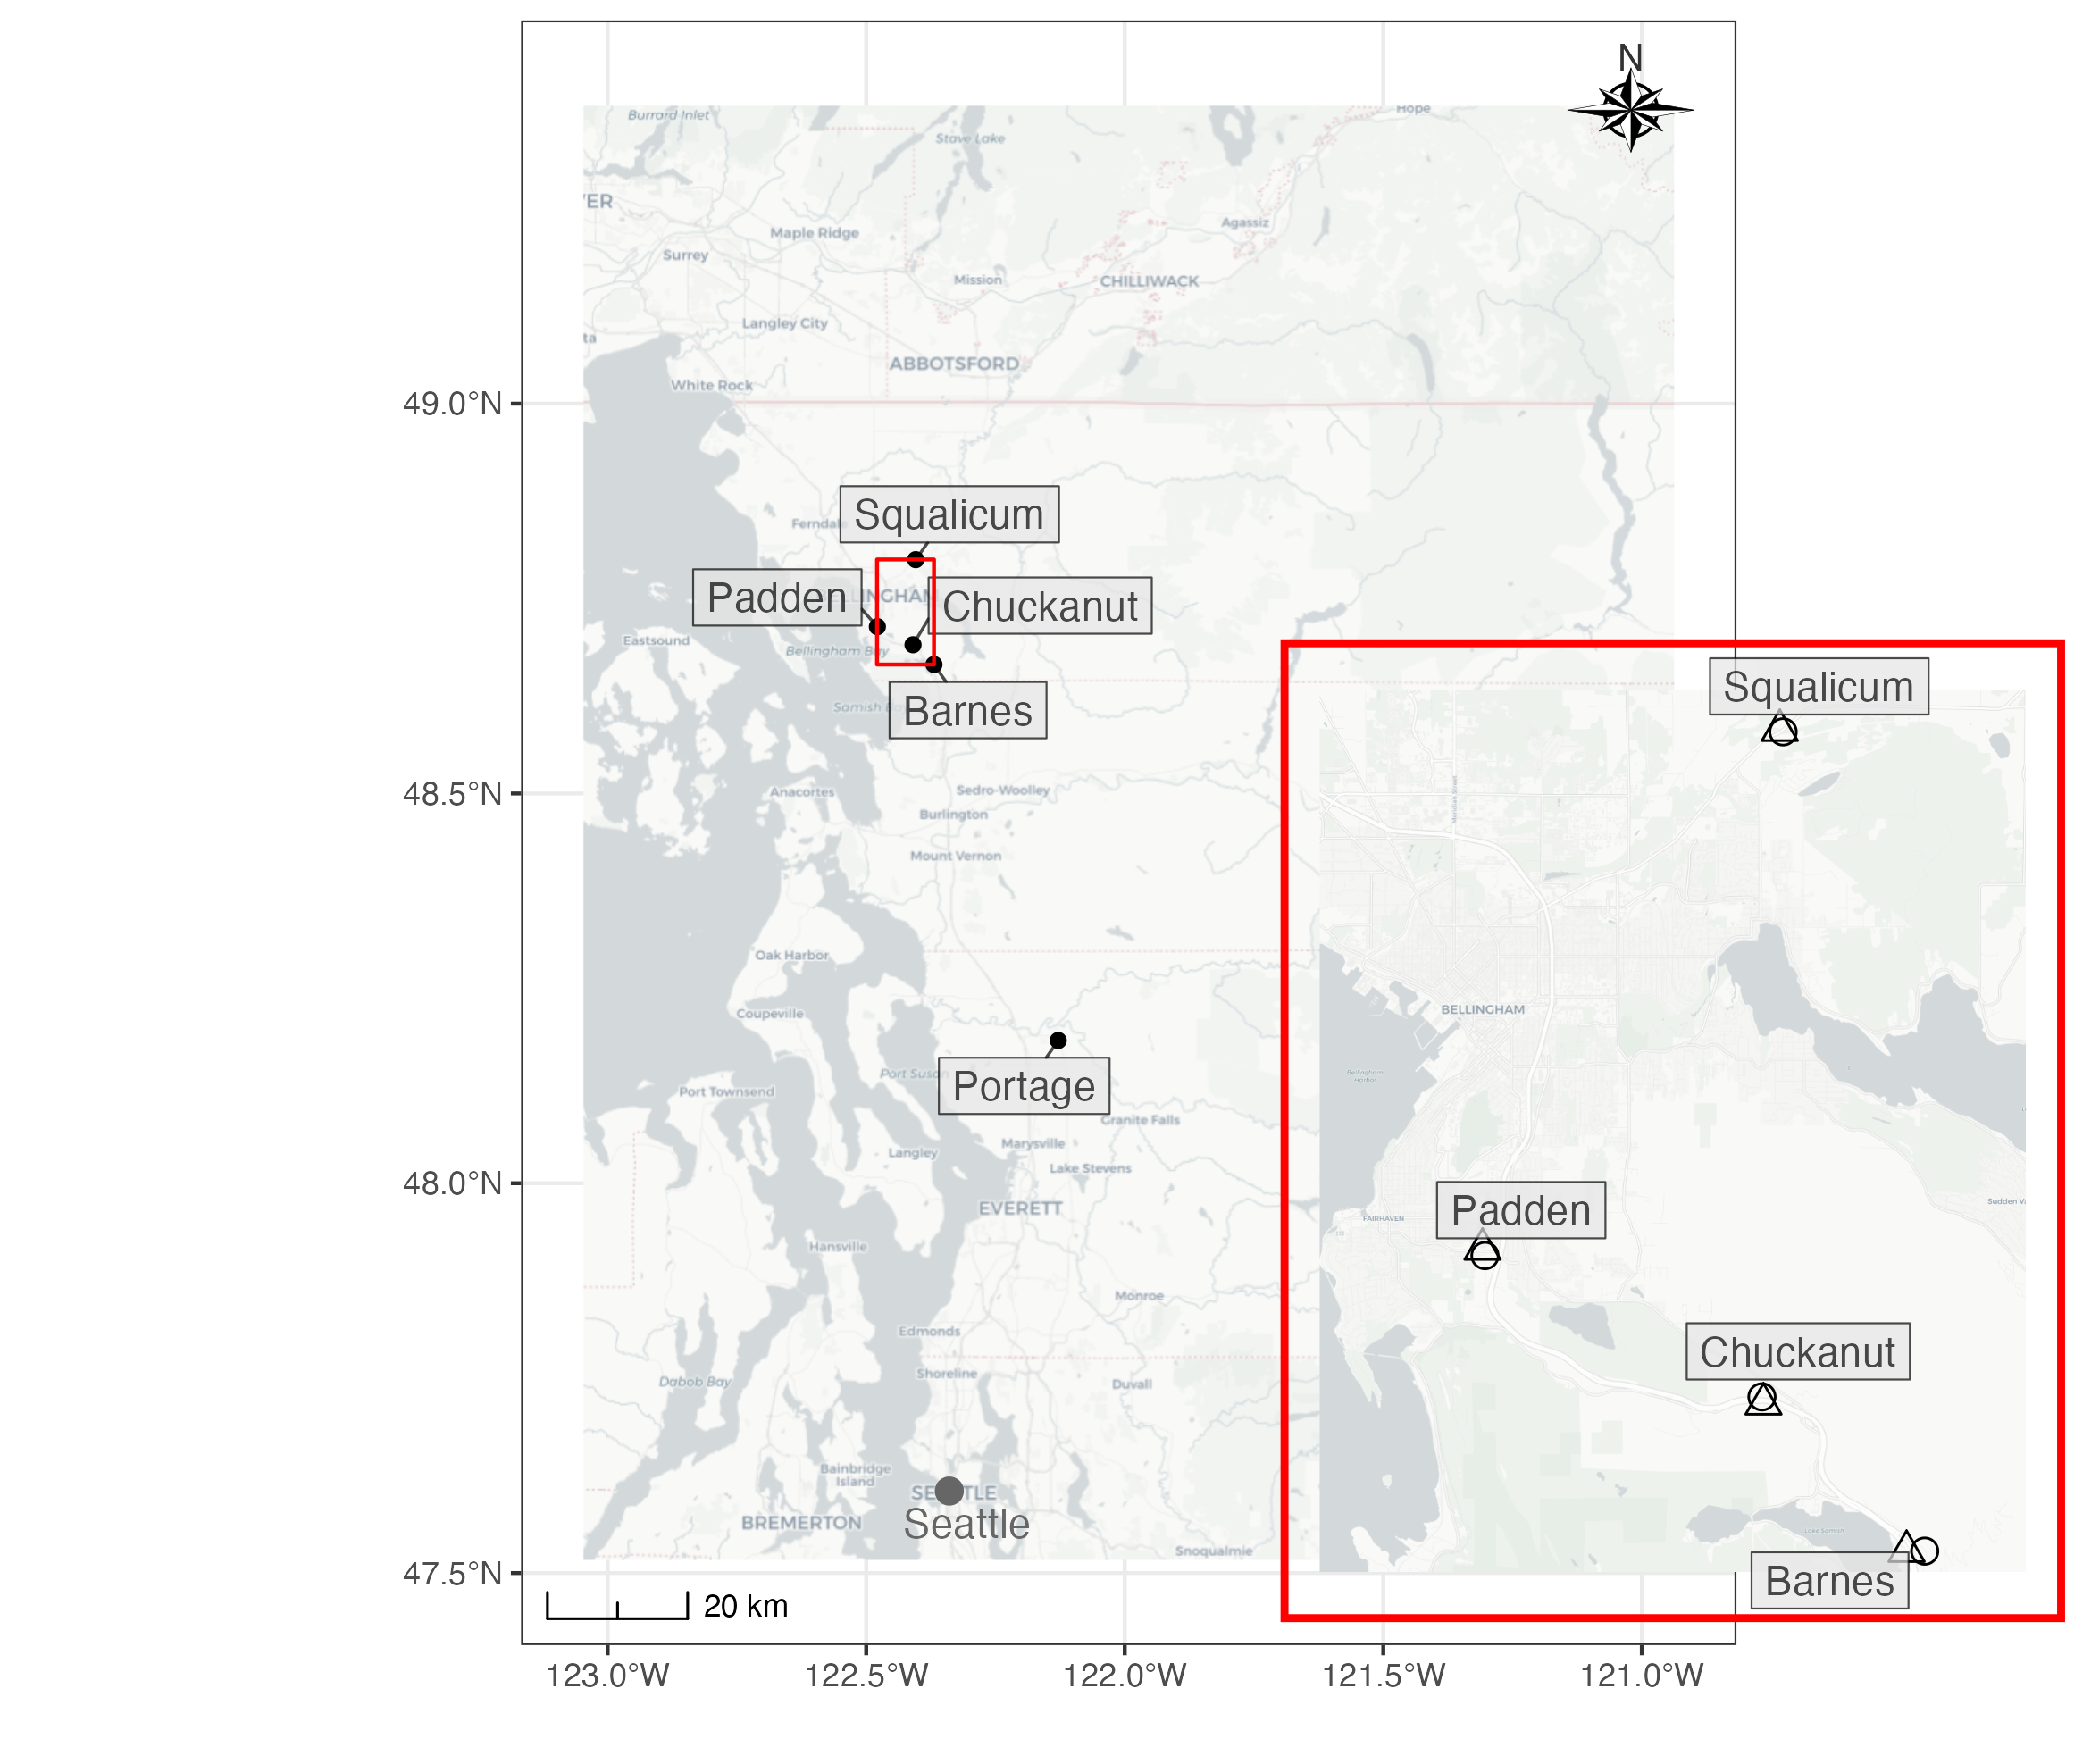
\includegraphics[width=0.5\textwidth,height=\textheight]{../Output/Figures/SiteMap.png}
\caption{Map of sampling locations near Bellingham,
Washington.\label{fig:map}}
\end{figure}

At each sampling station (N=2, upstream and downstream of a culvert) at
each creek (N = 5) in each month (N = 12), we collected three 2-liter
water samples, for a total of 360 samples. Water samples were collected
using Smith Root's eDNA Backpack (Thomas et al., 2018), a portable
pumping-and-filtering device set to filter at 1 L/min at 82.7 kPa (12
psi). In some months, less than 2 L of water was filtered due to
clogging (Supplemental Table 1). Water samples were filtered through
5\(\mu\)m self-preserving filters (Smith Root, Vancouver, WA) using
single-use inlet tubes, which were then dried, and kept at room
temperature until DNA extraction within 1 month of collection (Thomas et
al., 2019).

Water discharge varied throughout the year, with lowest discharge in
summer months and highest discharge in winter months (Figure 2). Flow
gauges maintained by USGS were used for Padden Creek, Chuckanut Creek,
and Squalicum Creek (U. S. Geological Survey, 1994). During the year of
sampling, the flow gauges at Chuckanut Creek and Squalicum Creek stopped
metering after a major flooding event. To find discharge rates for each
creek to correct eDNA concentrations by discharge, five years of
historical data (2015-2020) of the three creeks were used to generate a
monthly averaged correction factor based on Padden Creek. For the year
of sampling (2021-2022), the discharge rates used at Chuckanut and
Squalicum Creeks were estimated based on the correction factor from
Padden Creek (Supplemental Figure 1). No discharge data was available
for Portage Creek or Barnes Creek. Based on field sampling conditions,
the discharge from Padden Creek was used as a proxy for both Portage and
and Barnes as they were similar sizes and flow rates. Though in the year
of sampling, the discharge in Padden Creek ranged from no metered flow
to 23 m\textsuperscript{3}/s, the discharge on the dates of sampling
only reached a maximum of 1.3 m\textsuperscript{3}/s.

\begin{figure}
\centering
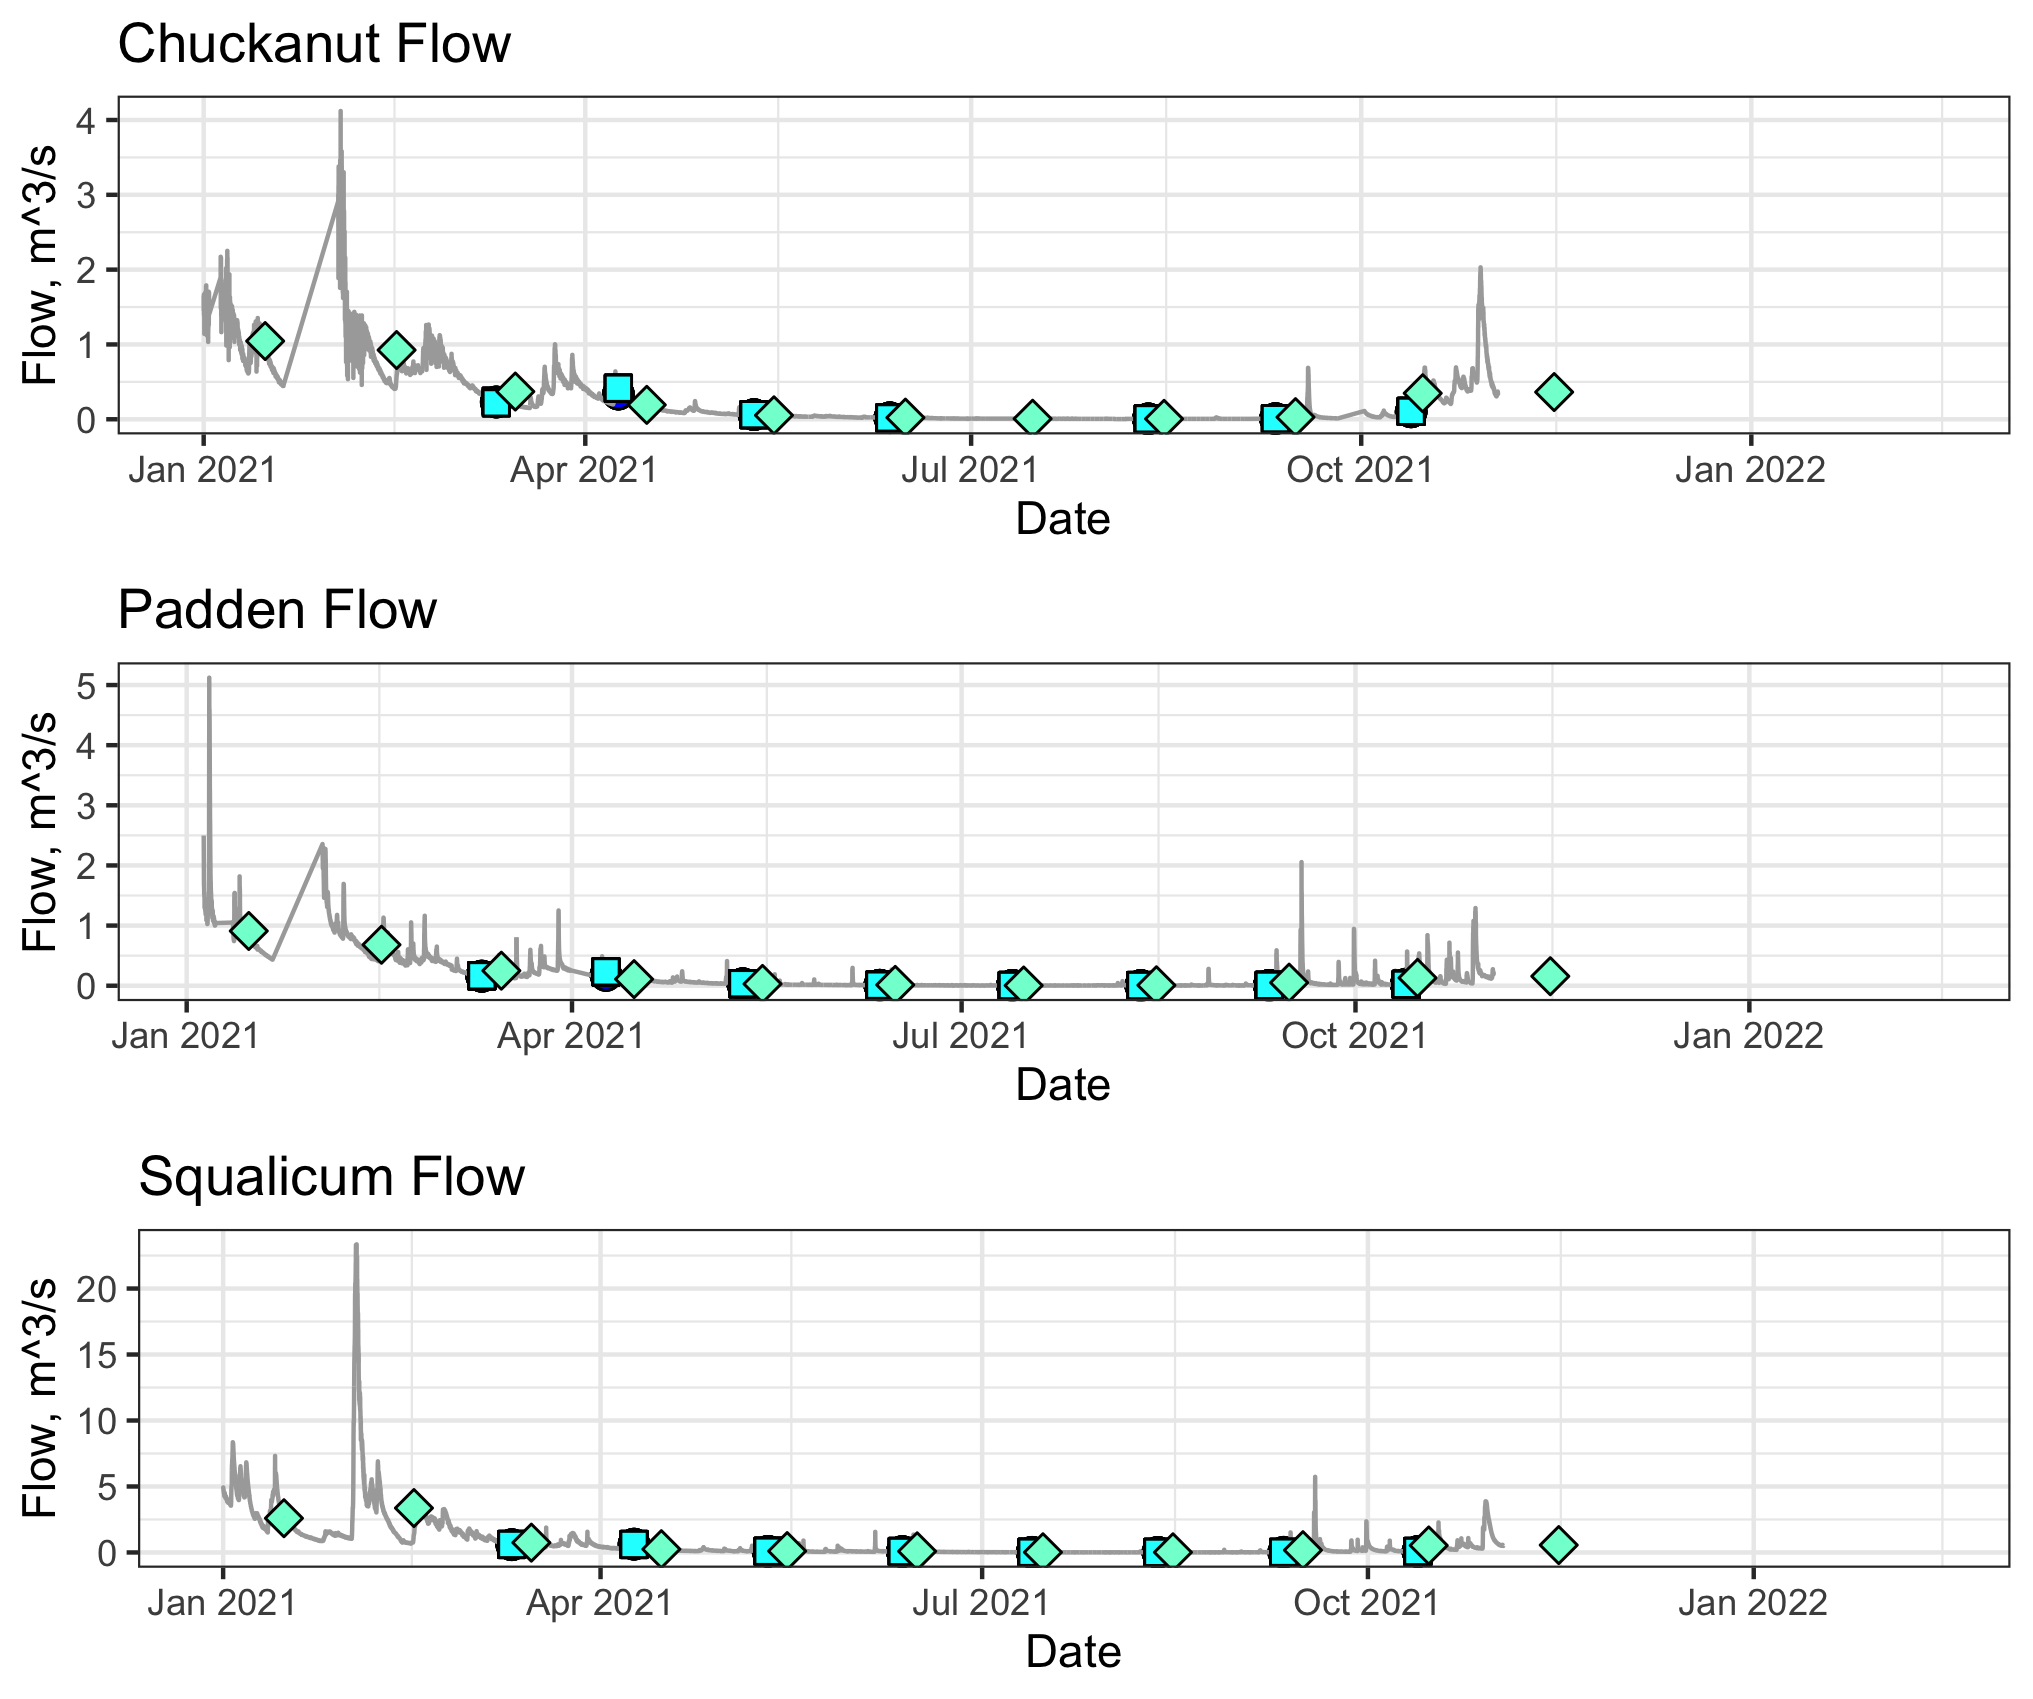
\includegraphics[width=0.5\textwidth,height=\textheight]{../Output/Figures/flow_gauges.png}
\caption{Discharge (m\textsuperscript{3}/s) in Padden, Chuckanut, and
Squalicum Creeks over the course of sampling. Open circles show the days
when sampling occurred. Gauges at Chuckanut and Squalicum Creek went
offline in November 2021 after a major storm event.\label{fig:flows}}
\end{figure}

Additionally, in the creek of interest, Padden Creek, \emph{O. mykiss}
(rainbow trout) were stocked in Lake Padden, approximately 1.5 km
upstream of the sampling sites. Occasionally, cutthroat trout (\emph{O.
clarkii}) and kokanee salmon (\emph{O. nerka}) have been stocked in the
past as well. During the course of the study, a total of 10,000 rainbow
trout were stocked in April and May 2021, 30,000 kokanee salmon were
stocked in May 2021, and 10,000 cutthroat trout were stocked in January
2021 (Supplemental Figure 2).

\hypertarget{dna-extraction-amplification-sequencing}{%
\subsubsection{DNA Extraction, Amplification,
Sequencing}\label{dna-extraction-amplification-sequencing}}

All molecular work was performed at the University of Washington.
Benchtops were cleaned with 10\% bleach for 10 minutes and then wiped
with 70\% ethanol. Molecular work was separated onto pre- and post-PCR
benches; all DNA extractions and PCR preparation was conducted on a
bench where no PCR product was handled. DNA was extracted from half of
each filter using a Qiashredder column (Qiagen, USA) and the DNEasy
Blood and Tissue Kit (Qiagen, USA) with an overnight incubation
(Supplemental Text 1, Thomas et al. (2019)), such that the effective
filtering effort was 1 L/sample; the remaining half of each filter was
archived at -20\degree C. Extracts were eluted in 100 \(\mu\)L of
molecular grade water, quantified via Qubit (Invitrogen, USA) and stored
at -20\degree C until PCR amplification within 2 months of extraction.

For metabarcoding, we targeted a \textasciitilde170 bp hypervariable
region of the mitochondrial DNA 12S rRNA gene for PCR amplification
(MiFish; Miya et al.~2015), but using modified primer sequences as given
in Praebel and Wangensteen {[}cite{]} and including the Illumina Nextera
overhang sequences for subsequent indexing. The primers used were as
follows: F 5'
\emph{TCGTCGGCAGCGTCAGATGTGTATAAGAGACAG}GCCGGTAAAACTCGTGCCAGC 3', R 5'
\emph{GTCTCGTGGGCTCGGAGATGTGTATAAGAGACAG}CATAGTGGGGTATCTAATCCCAGTTTG 3'
(\emph{italics} indicate Nextera overhang). The final reaction recipe
and cycling conditions can be found in Supplemental Text 1. Each month
of samples was amplified on a single plate with the addition of a no
template control (NTC; molecular grade water in lieu of template) and a
positive control (genomic DNA from kangaroo). After PCR amplification,
PCR products were visualized on a 1-2\% gel. If no band was present for
a given sample, a new amplification was attempted with extracts diluted
1:10 iteratively until a band was detected. PCR products were
size-selected and cleaned using MagBind Beads (Omega Biotek, USA) at a
sample:beads ratio of 1.2. Bead-cleaned PCR products were eluted in 30
\(\mu\)L of molecular grade water and quantified via Qubit (Invitrogen,
USA).

A indexing PCR reaction added a unique index to each sample using
Nextera indices (Illumina, USA) to allow pooling multiple samples onto
the same sequencing run (See Supplemental Text 1 for details). Indexed
PCR products were also size-selected and purified using MagBind Beads
(Omega Biotek, USA) at a sample:beads ratio of 0.8. Bead-cleaned PCR
products were eluted in 30 \(\mu\)L of molecular grade water and
quantified via Qubit. Indexed and bead-cleaned products were normalized
before pooling into libraries, which were subsequently quantified via
Qubit and visualized on a Bioanalyzer (Agilent, USA) before sequencing.
Samples were randomized in 3-month blocks and each block split across 3
sequencing runs, for a total of 12 MiSeq runs. The loading concentration
of each library was 4-8 pM and 5-20\% PhiX was included depending on the
composition of the run (Supplemental Table 2).

\hypertarget{bioinformatics}{%
\subsubsection{Bioinformatics}\label{bioinformatics}}

After sequencing, bioinformatic analyses were conducted in R (R Core
Team, 2017). Information about the bioinformatics pipeline is included
in the supplement (Supplemental Text 1). Briefly, primer sequences were
removed using Cutadapt (Version 1.18) (Martin, 2011) before dada2
(Callahan et al., 2016) trimmed, filtered, merged paired end reads, and
generated amplicon sequence variants (ASVs). Taxonomic assignment was
conducted via the insect package (Wilkinson et al., 2018) using a tree
generated by the developers for the MiFish primers that was last updated
in November 2018. Only species level assignments from insect were
retained and ASVs not annotated or not annotated to species level were
then checked against the NCBI nucleotide database using BLAST+ (Camacho
et al., 2009). Query sequences that matched a single species at
\textgreater95\% identity were retained.

In total, sequencing runs generated \textasciitilde42 million reads
across all environmental samples (12 months x 2 stations x 5 creeks x 3
biological replicates = 360 filters) and 27 mock community samples (3
communities x 9 replicates {[}6 even, 3 skewed proportions{]}) for
calibration (see below). After quality-filtering and merging all runs,
\textasciitilde33 million reads remained from \textasciitilde21,000
amplicon sequence variants (ASVs) in the environmental samples, of which
\textasciitilde81\% of reads and \textasciitilde2\% of ASVs were
annotated to species level (per sample: mean = 78\%, median = 88\%, min
= 0\%, max = 99.99\% of reads annotated). We only focus on the
metabarcoding data from four salmonids for the remainder of this paper.
The four salmonids represent \textasciitilde55\% of all enviromental
reads and \textasciitilde68\% of the annotated reads found in
environmental samples.

In the mock community samples, 98.65\% of the \textasciitilde5 million
reads after quality filtering were annotated to species level.
Importantly, the particular target salmonid ASVs in the mock communities
were found in environmental samples, unambiguously linking the taxa in
calibration samples with those in environmental samples. The most common
salmonid species found in the environmental samples was \emph{O.
clarkii} (cutthroat trout), which was found in \textasciitilde90\% of
samples, followeb by \emph{O. kisutch} found in \textasciitilde60\% of
samples, then \emph{O. mykiss} found in \textasciitilde40\% of samples,
and finally \emph{O. nerka} found in \textasciitilde5\% of samples. Not
only was \emph{O. clarkii} found in the majority of environmental
samples, but also \textasciitilde63\% of samples across all times,
creeks, and stations had at least 50\% of reads assigned to \emph{O.
clarkii}.

\hypertarget{quantitative-pcr-and-inhibition-testing}{%
\subsubsection{Quantitative PCR and Inhibition
Testing}\label{quantitative-pcr-and-inhibition-testing}}

We quantified cutthroat trout (\emph{O. clarkii}) DNA in each sample,
targeting a 114 bp fragment of the cytochrome b gene with a qPCR assay
(Duda et al., 2021). The primer/probe sequences were: F 5'
CCGCTACAGTCCTTCACCTTCTA 3', R 5' GATCTTTGTATGAGAAGTAAGGATGGAA 3', P 5'
6FAM-TGAGACAGGATCCAAC-MGB-NFQ 3'. The qPCR assay was multiplexed with
TaqMan Exogenous Internal Positive Control Reagents (EXO-IPC) (Applied
Biosystems, USA) to check for the presence of PCR inhibitors (Duda et
al., 2021). The EXO-IPC mix includes the primers and probe for the
EXI-IPC DNA, with the probe having a VIC reporter, allowing it to be
multiplexed with the \emph{O. clarkii} assay, which has a FAM reporter.
Each DNA sample was run in triplicate; the final recipe and
thermocycling conditions can be found in Supplemental Text 1. All qPCRs
were conducted on an Applied Biosystems StepOnePlus thermocycler.

Each plate included a 8-point standard curve created using synthetic DNA
(gBlocks) at the following concentrations: 100,000 copies/\(\mu\)L,
10,000 copies/\(\mu\)L, 1,000 copies/\(\mu\)L, 100 copies/\(\mu\)L, 10
copies/\(\mu\)L, 5 copies/\(\mu\)L, 3 copies/\(\mu\)L, 1 copy/\(\mu\)L
Additionally, six no template controls (NTCs) were included on each
plate: 3 with the IPC DNA mix and 3 with molecular grade water instead
of template or IPC DNA mix. Plates were re-run if efficiency as
determined by the standard curve was outside of the range of 90-110\%.

To check for inhibition, the cycle threshold (Ct) value determined for
the EXO-IPC assay from the NTC was compared to the Ct value for the
EXO-IPC assay in each of the environmental samples. If the Ct value was
\textgreater0.5 Ct values from the mean Ct for the NTCs, the sample was
deemed inhibited and diluted 1:10 and re-assayed until the Ct value fell
within the accepted range. The majority of environmental samples (65\%)
were inhibited and accordingly diluted for analysis. In 75\% of
inhibited samples, a 1:10 dilution remedied the inhibition, but some
samples required dilution by a factor of up to 1000.

All qPCR data was processed in R using Stan (Stan Development Team,
2022), relating environmental samples to the standard curve via a linear
model (Figure \ref{fig:conceptualfig}, blue boxes). We amended the
standard linear regression model to more realistically capture the
behavior of qPCR observations, accommodating non-detections as a
function of underlying DNA concentration, and letting the standard
deviation vary with the mean (lower-concentration samples had more
uncertainty). See McCall et al. (2014) and Shelton et al. (2019) for
similar models; see Supplemental Text 2 for full statistical details.
Subsequent analysis corrected for sample-specific dilution if found
inhibited and corrected for any variation in water-volume filtered
during sample collection.

\hypertarget{quantitative-metabarcoding}{%
\subsubsection{Quantitative
Metabarcoding}\label{quantitative-metabarcoding}}

Here, we used a mock community to determine the species-specific
amplification efficiencies for each salmonid in the study. Briefly, we
constructed three communities with known proportions of starting DNA
from different species (total DNA as measured by Qubit). Each community
was constructed with an even proportion of each species and a skewed
proportion. We sequenced these communities using the same metabarcoding
primers and thermocycling conditions above and then can determine the
species-specific amplification rates given the discrepancy between the
known starting proportion and the proportion of reads after sequencing.
These mock community data are then used to correct the sequencing reads
from the environmental samples to estimate the starting DNA proportions
of each species in environmental samples, which is the metric of
interest (Figure 3, green boxes). See Shelton et al. (2022) and
Supplemental Text 2 for more information. The intercalibration of the
mock community samples demonstrates the rank order of ampliciation
efficiencies for salmonids (Supplemental Figures 3 and 4). \emph{O.
clarkii} and \emph{O. nerka} had similar amplification efficiencies,
both of which were higher than \emph{O. mykiss} and \emph{O. kisutch},
which had the lowest amplification efficiency.

Calibrated metabarcoding analysis yielded quantitative estimates of the
proportions of species' DNA in environmental samples prior to PCR. We
then converted these proportions into absolute abundances by expansion,
using the qPCR results for our reference species, \emph{O. clarkii}. We
estimated the total amplifiable salmonid DNA in environmental sample
\(i\) as
\(DNA_{salmonid_{i}} = \frac{[qPCR_{reference_{i}}]}{Proportion_{reference_{i}}}\),
and then expanded species' proportions into absolute concentrations by
multiplying these sample-specific total concentrations by individual
species' proportions, such that for species \(j\) in sample \(i\),
\(DNA_{i,j} = DNA_{salmonid_{i}} * Proportion_{i,j}\). Finally, we
convert from DNA concentration {[}copies/L{]} to a mass flow rate
{[}copies/s{]} after multiplying by the discharge of each creek
{[}m\textsuperscript{3}/s{]} (Figure \ref{fig:conceptualfig}, solid
purple boxes).

\begin{figure}
\centering
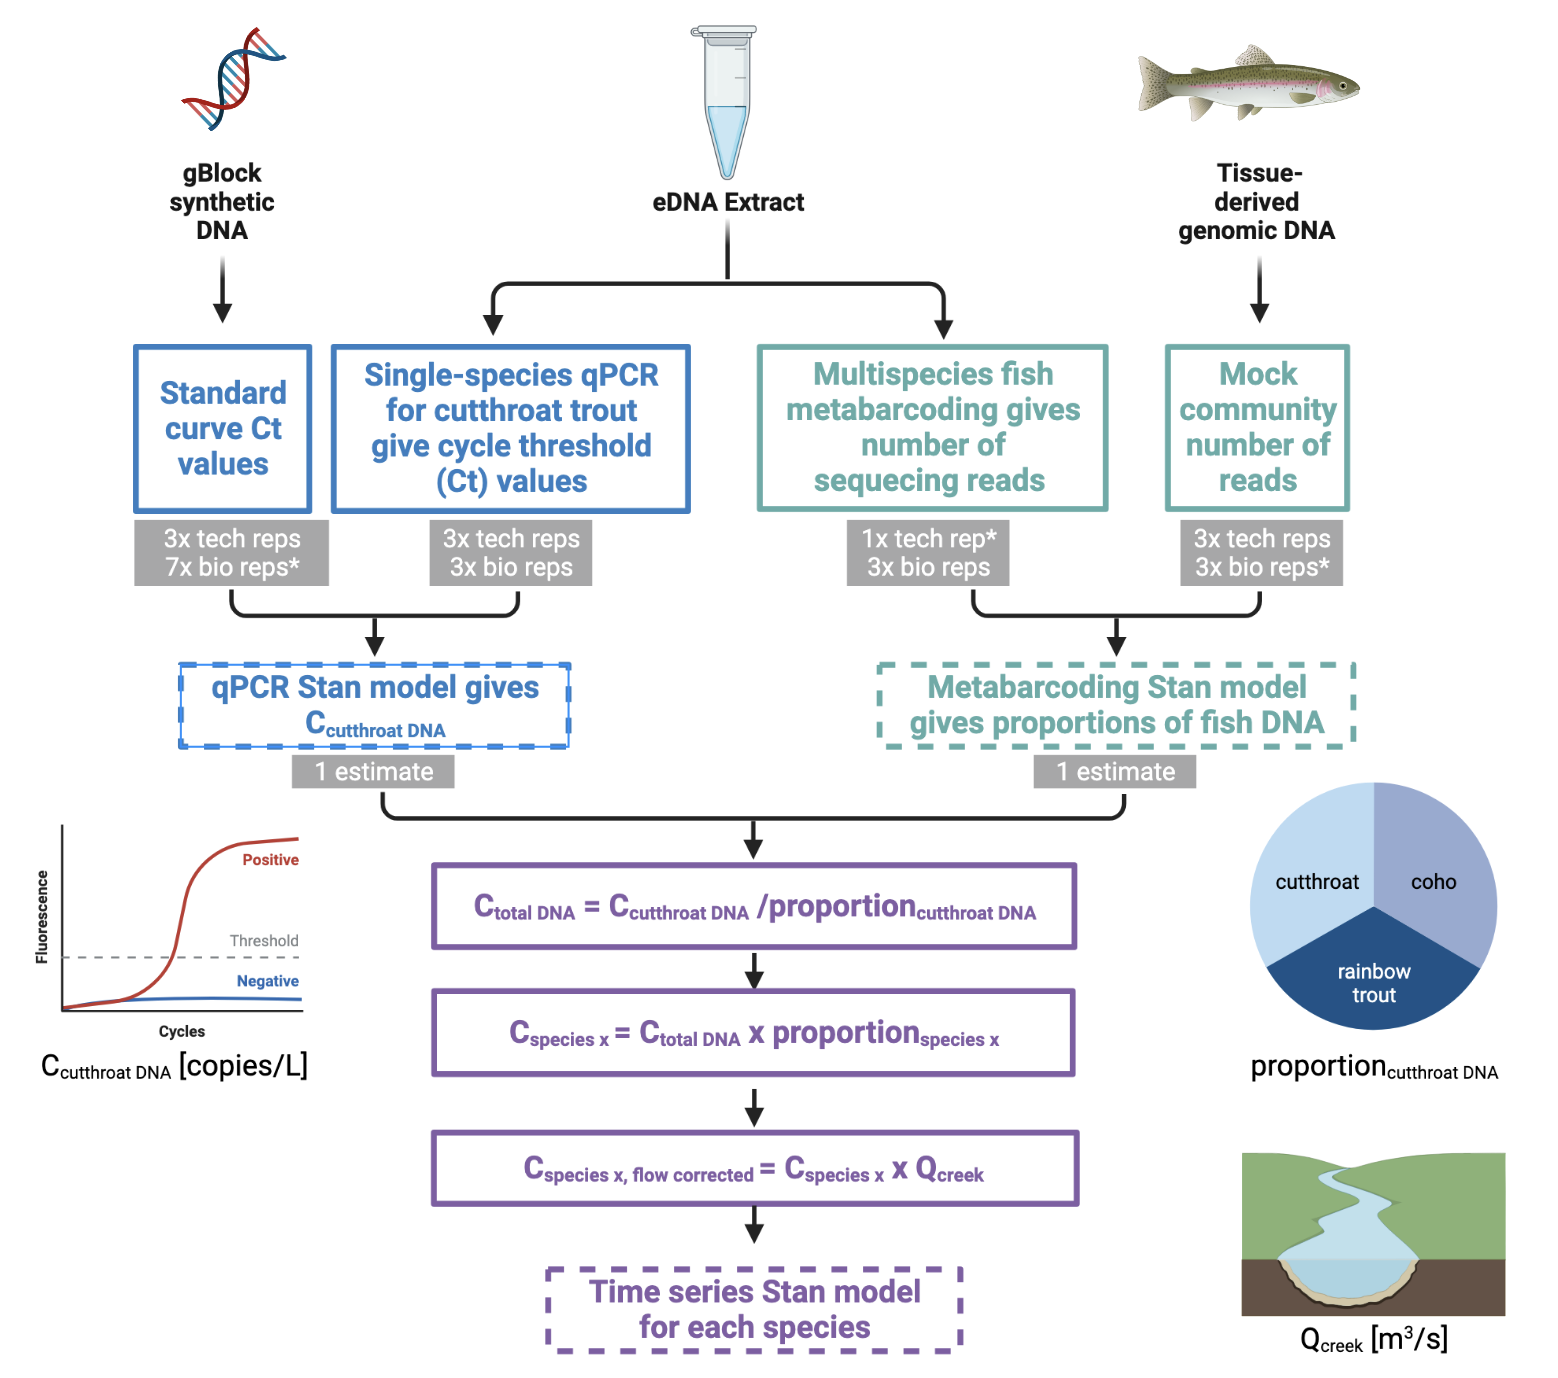
\includegraphics[width=0.75\textwidth,height=\textheight]{../Output/Figures/conceptual_figure.png}
\caption{Conceptual figure of different datasets and models used for
analyses.\label{fig:conceptualfig}}
\end{figure}

\hypertarget{estimating-the-effects-of-culvert-replacement-and-of-culverts-themselves}{%
\subsubsection{Estimating the Effects of Culvert Replacement and of
Culverts
Themselves}\label{estimating-the-effects-of-culvert-replacement-and-of-culverts-themselves}}

Consistent with the asymmetrical BACI study design, we generated data
from our four control creeks as context against which to compare the
observations in Padden Creek, our treatment creek. Recognizing that
these observations are autocorrelated in time, we use an AR(1)
autocorrelation model, implemented in Stan via R, to capture the
observed temporal trends. At time \(t\), the expected log-DNA
concentration for species \(j\) in creek \(i\) at station \(d\) is a
linear function of the DNA concentration for the same
species/creek/station at \(t-1\) (Equation \ref{eqn:ts}). We add an
index \(r\) to distinguish samples from creeks and time-points that had
not undergone culvert replacement (controls; \(r = 1\)) from those
samples in the treatment creek during and post-replacement (treatment;
\(r = 2\)).

\begin{align*}\label{eqn:ts}
 Y_{i,t,d,j} &\sim \mathcal{N}(\mu_{i,t,d,j},\,\sigma^{2})\\
\mu_{i,t,d,j} &= \alpha_{i,t,j} + \beta_{j}\mu_{i,t-1,d,j} + \gamma_{t,j,r} + \eta_{i,t,d,j}\tag{1}\\ 
\end{align*}

The model shares information across creeks and time-points via a
species-specific slope term \(\beta_{j}\), which reflects characteristic
degrees of autocorrelation for each species. Intercept \(\alpha\) varies
by time, creek, and species, capturing creek-level deviations from the
previous time-step.

The \(\gamma\) term explicitly captures the effect of culvert
replacement at time \(t\) for species \(j\). We define
\(\gamma_{r = 1} = 0\), such that the parameter estimates for samples
during and after replacement, \(\gamma_{r = 2}\), capture the effect of
culvert replacement relative to a baseline of zero.

Finally, for a given time/creek/species, the difference in log-DNA
concentration between upstream and downstream stations is calculated as
the difference between the parameter values of \(\eta\) for the two
stations. All samples share a species-specific observation-variance
term, \(\sigma_{j}\).

We fitted this model in a Bayesian framework using moderately
informative priors on all parameters, and confirmed model convergence
(\(\hat{R} < 1.01\)) across 3 chains and 2500 model iterations. See
statistical supplement (Supplemental Text 2) for prior values,
diagnostics, and full model details.

\hypertarget{results}{%
\subsection{Results}\label{results}}

\hypertarget{metabarcoding-and-quantitative-pcr}{%
\subsubsection{Metabarcoding and Quantitative
PCR}\label{metabarcoding-and-quantitative-pcr}}

After calibrating metabarcoding data using mock communities, we
estimated the salmonid composition across time points, creeks, and
stations (Figure \ref{fig:qm}). The culvert in one control creek
(Barnes) appeared to be nearly a total barrier to salmonid passage, with
salmonid eDNA detected upstream of the culvert at only three time
points, in contrast to being detected at every time point in the
downstream station of the same creek. The other four creeks had no such
pattern associated with the culverts, suggesting that fish passage may
have been possible in each case.

\begin{figure}
\centering
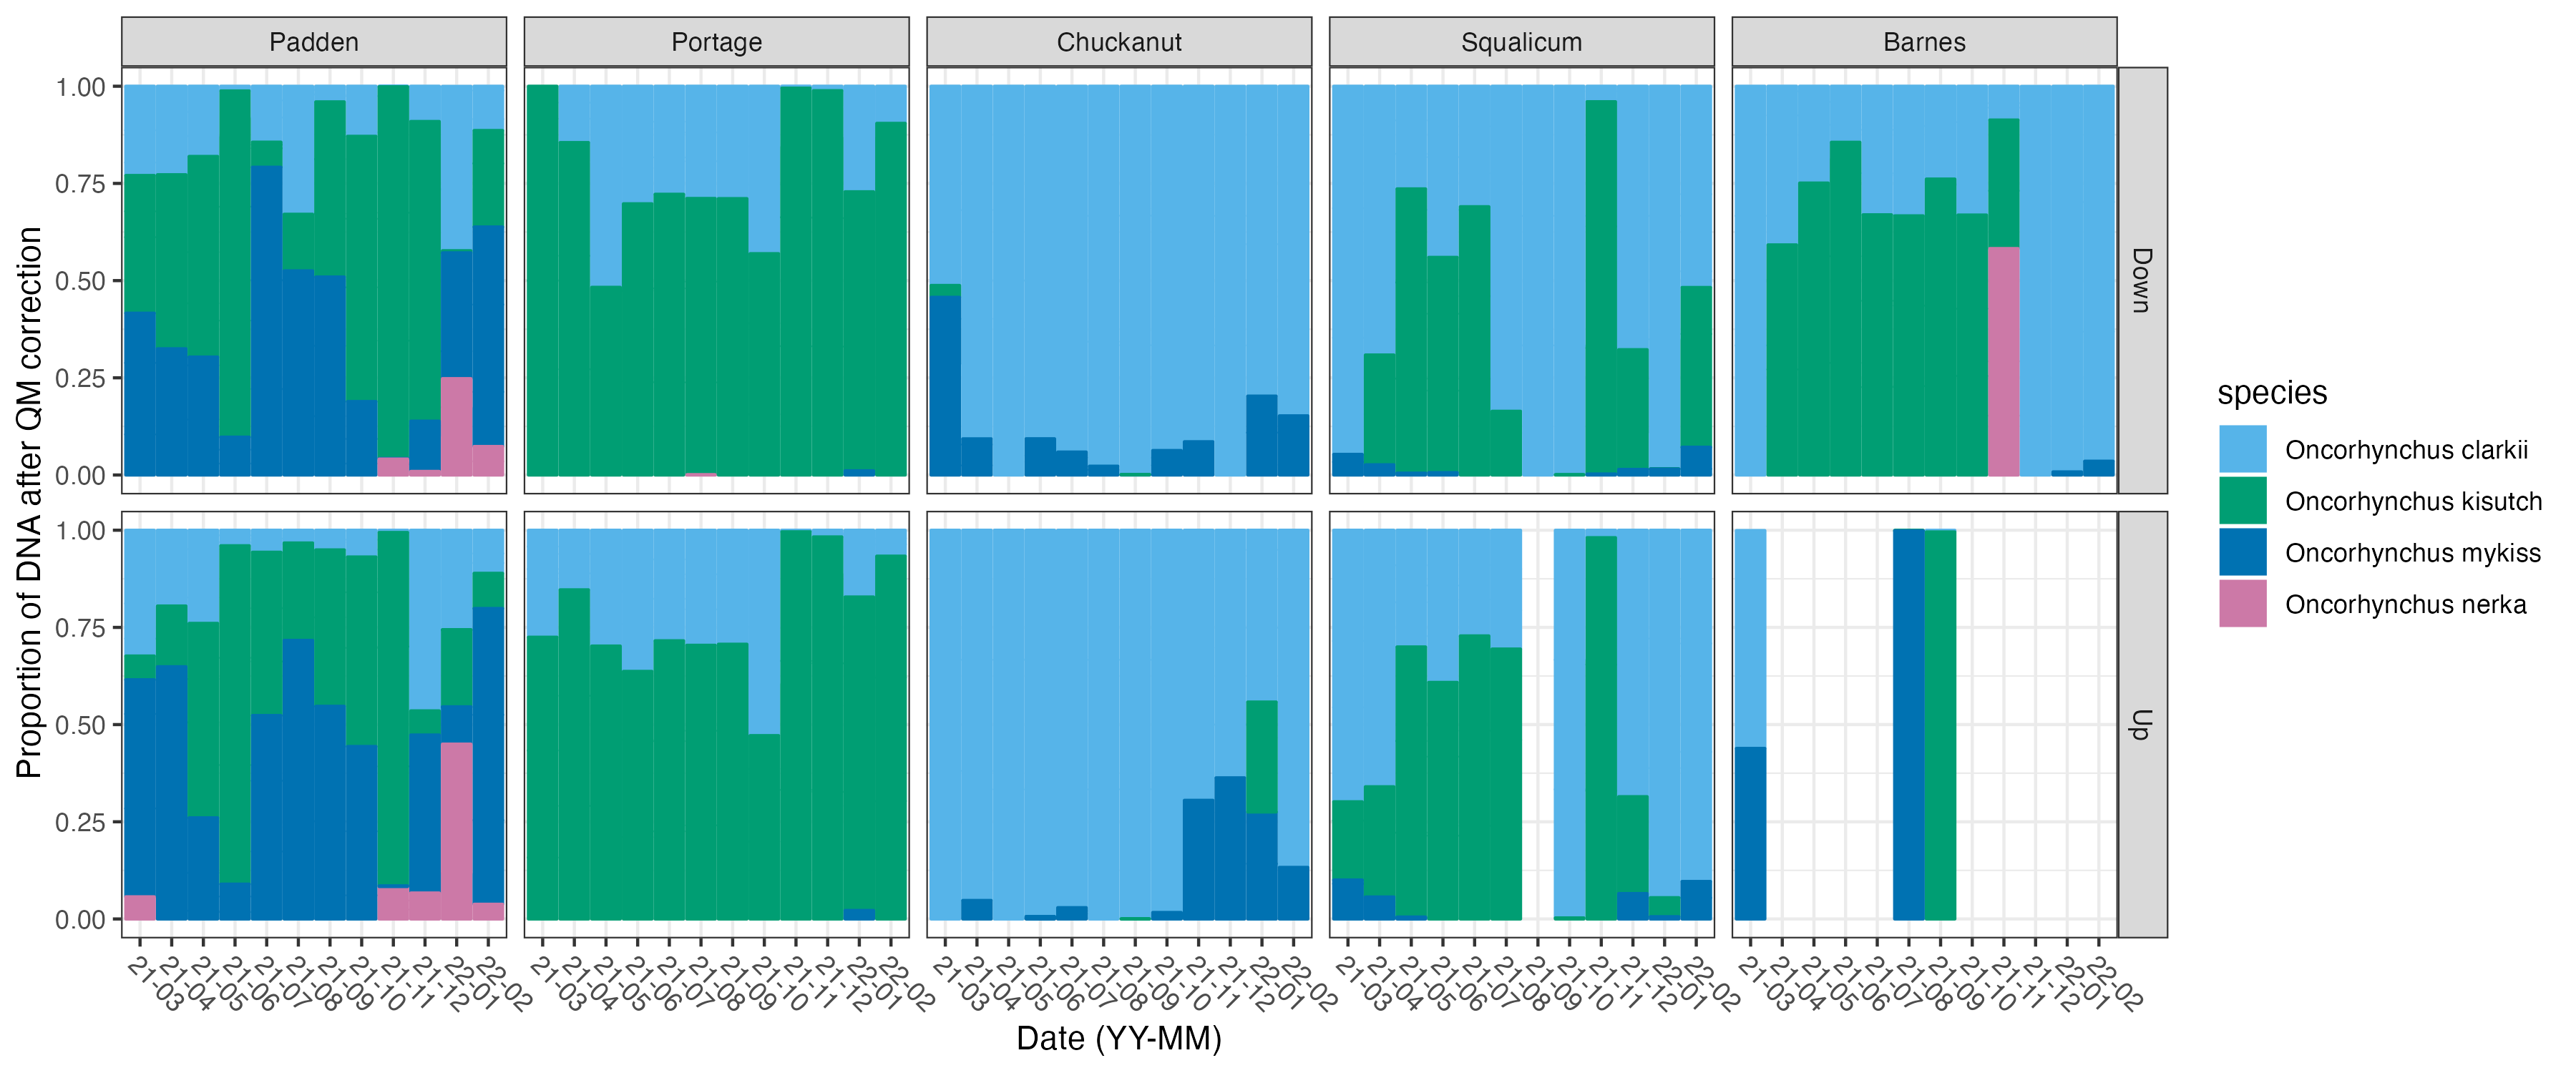
\includegraphics[width=0.9\textwidth,height=\textheight]{../Output/Figures/20221123_proportions_after_qm.png}
\caption{Compositions of salmonid DNA as determined by metabarcoding
after correction for amplification bias. Note that no sampling occurred
in September 2021 at Squalicum Creek becuase the creek was dry. The
empty bars in the Barnes upstream sites indicate that no salmonid DNA
was found at those time points.\label{fig:qm}}
\end{figure}

All environmental samples were quantified for absolute concentrations of
cutthroat trout DNA across 30 plates, resulting in 280 samples
(\textasciitilde80\%) with a positive detection in at least 1 of 3
technical replicates. The modeled output of cutthroat trout DNA
concentrations, ranged from 10 copies/L to 1,377,656 copies/L, with a
mean value of 57,529 copies/L (Figure \ref{fig:qpcr}).

\begin{figure}
\centering
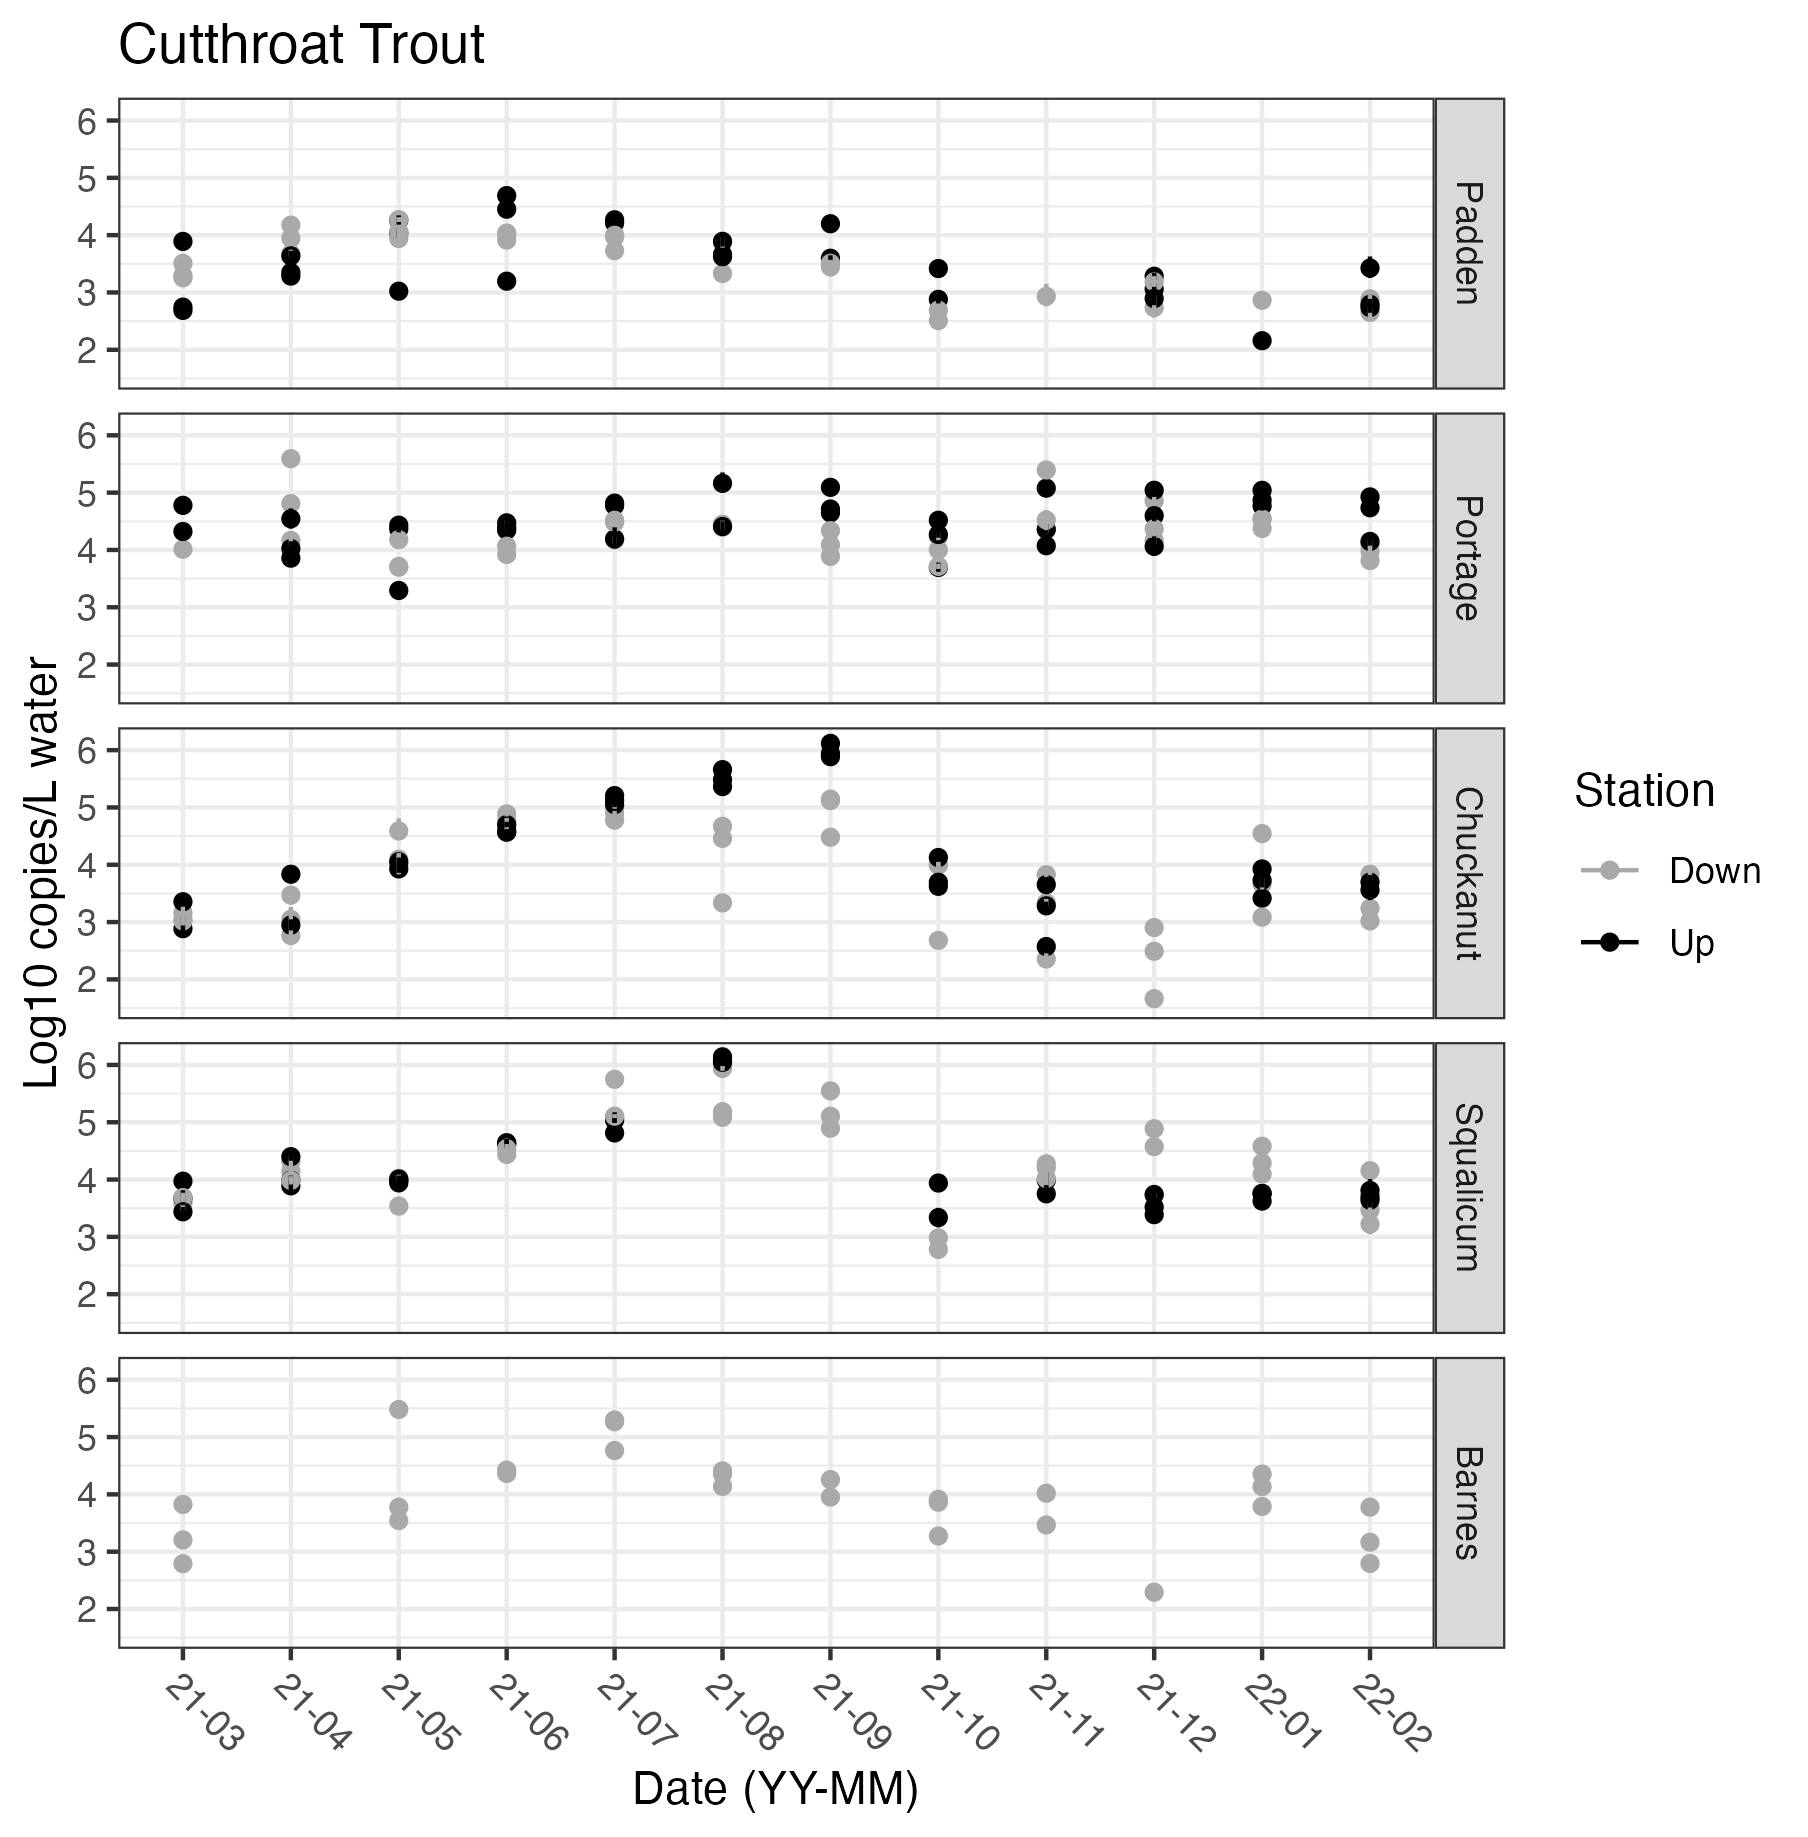
\includegraphics[width=0.6\textwidth,height=\textheight]{../Output/Figures/20221129_modeled_cut_qpcr_updown.png}
\caption{Absolute concentration (copies/L of water) of \emph{O. clarkii}
(cutthroat trout) as measured by qPCR.\label{fig:qpcr}}
\end{figure}

We combined compositional information from metabarcoding with absolute
concentrations for our reference species, \emph{O. clarkii}, from the
qPCR to estimate the total concentration of DNA for each species.

\hypertarget{trends-in-abundance}{%
\subsubsection{Trends in Abundance}\label{trends-in-abundance}}

The joint time-series model shared information across stations and
creeks; consequently, data from one of the control creeks (Barnes) could
not be included because of the total absence of salmonids upstream of
its culvert. However, data from the remaining creeks characterized
trends in the other four target species well (Figure \ref{fig:ts}).

\begin{figure}
\centering
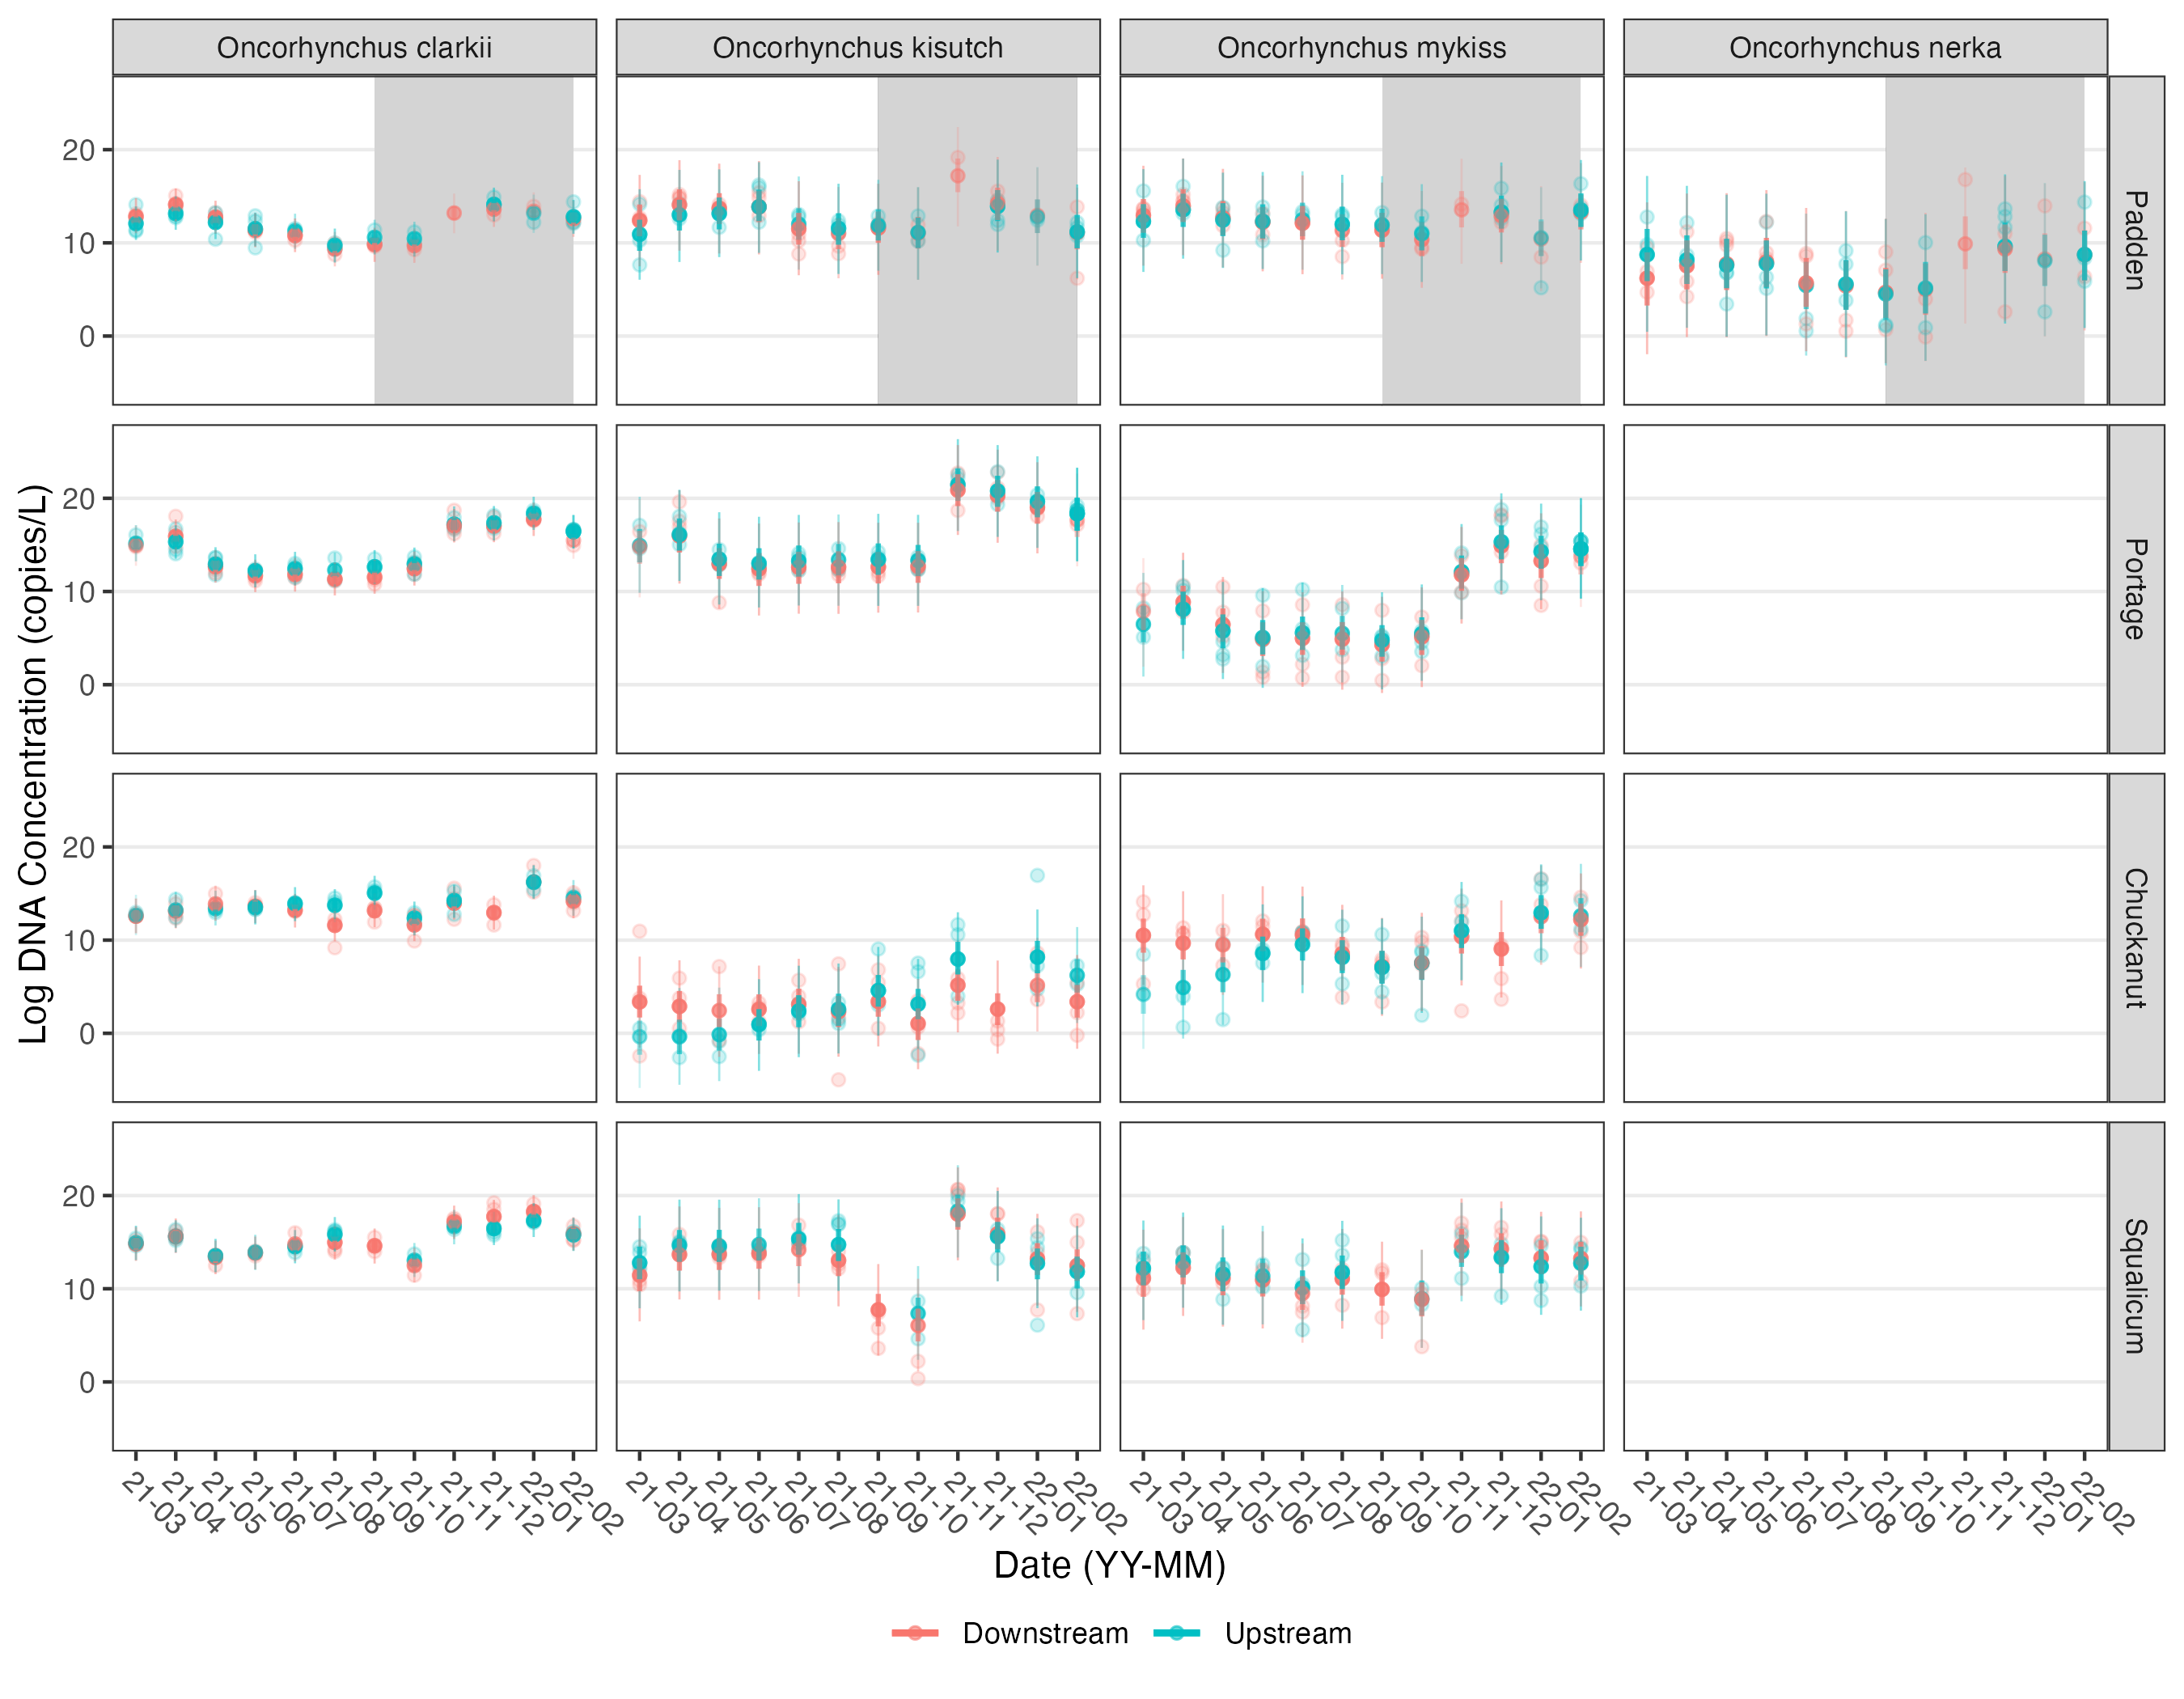
\includegraphics[width=0.6\textwidth,height=\textheight]{../Output/Figures/20221129_multispeciesTrends_flowcorrected.png}
\caption{Trends across creeks and across time for each of three salmonid
species as estimated by eDNA analysis. Light-colored dots are posterior
means derived by expanding the calibrated metabarcoding proportions as
described in the main text; darker-colored dots are posterior means for
the time-series model of the same. Colors indicate station upstream or
downstream of an under-road culvert. 75\% and 95\% posterior CI plotted
for each time point. Grey shading indicates the time period in which the
culvert in the treatment creek (Padden Creek) was
replaced.\label{fig:ts}}
\end{figure}

\hypertarget{effects-of-culverts}{%
\subsubsection{Effects of Culverts}\label{effects-of-culverts}}

Before considering the effect of construction, the difference in
abundance trends between upstream and downstream stations (Figure
\ref{fig:ts} demonstrate that the culverts themselves have some effect,
but not a large effect on the salmonid species surveyed. Summarizing
over all species, all creeks, the effect was largest during the dry
periods of summer (July, August, and September), when flows were at a
minimum and the connectivity between upstream and downstream was low
(Figure \ref{fig:culverts}). Salmonid species were higher upstream than
downstream during this period, with mean upstream DNA about 10\% higher
concentration than downstream DNA Individual species' patterns were
similar, indicating that there is not a species-specific effect where
culverts block the passage of some salmon but not others (Supplemental
Figure 5). A notable exception is \emph{O. kisutch} in Chuckanut Creek,
at some point reaching over 50\% higher concentration upstream than
downstream. Padden Creek and Squalicum Creek had the lowest percent
difference over the course of the year.

\begin{figure}
\centering
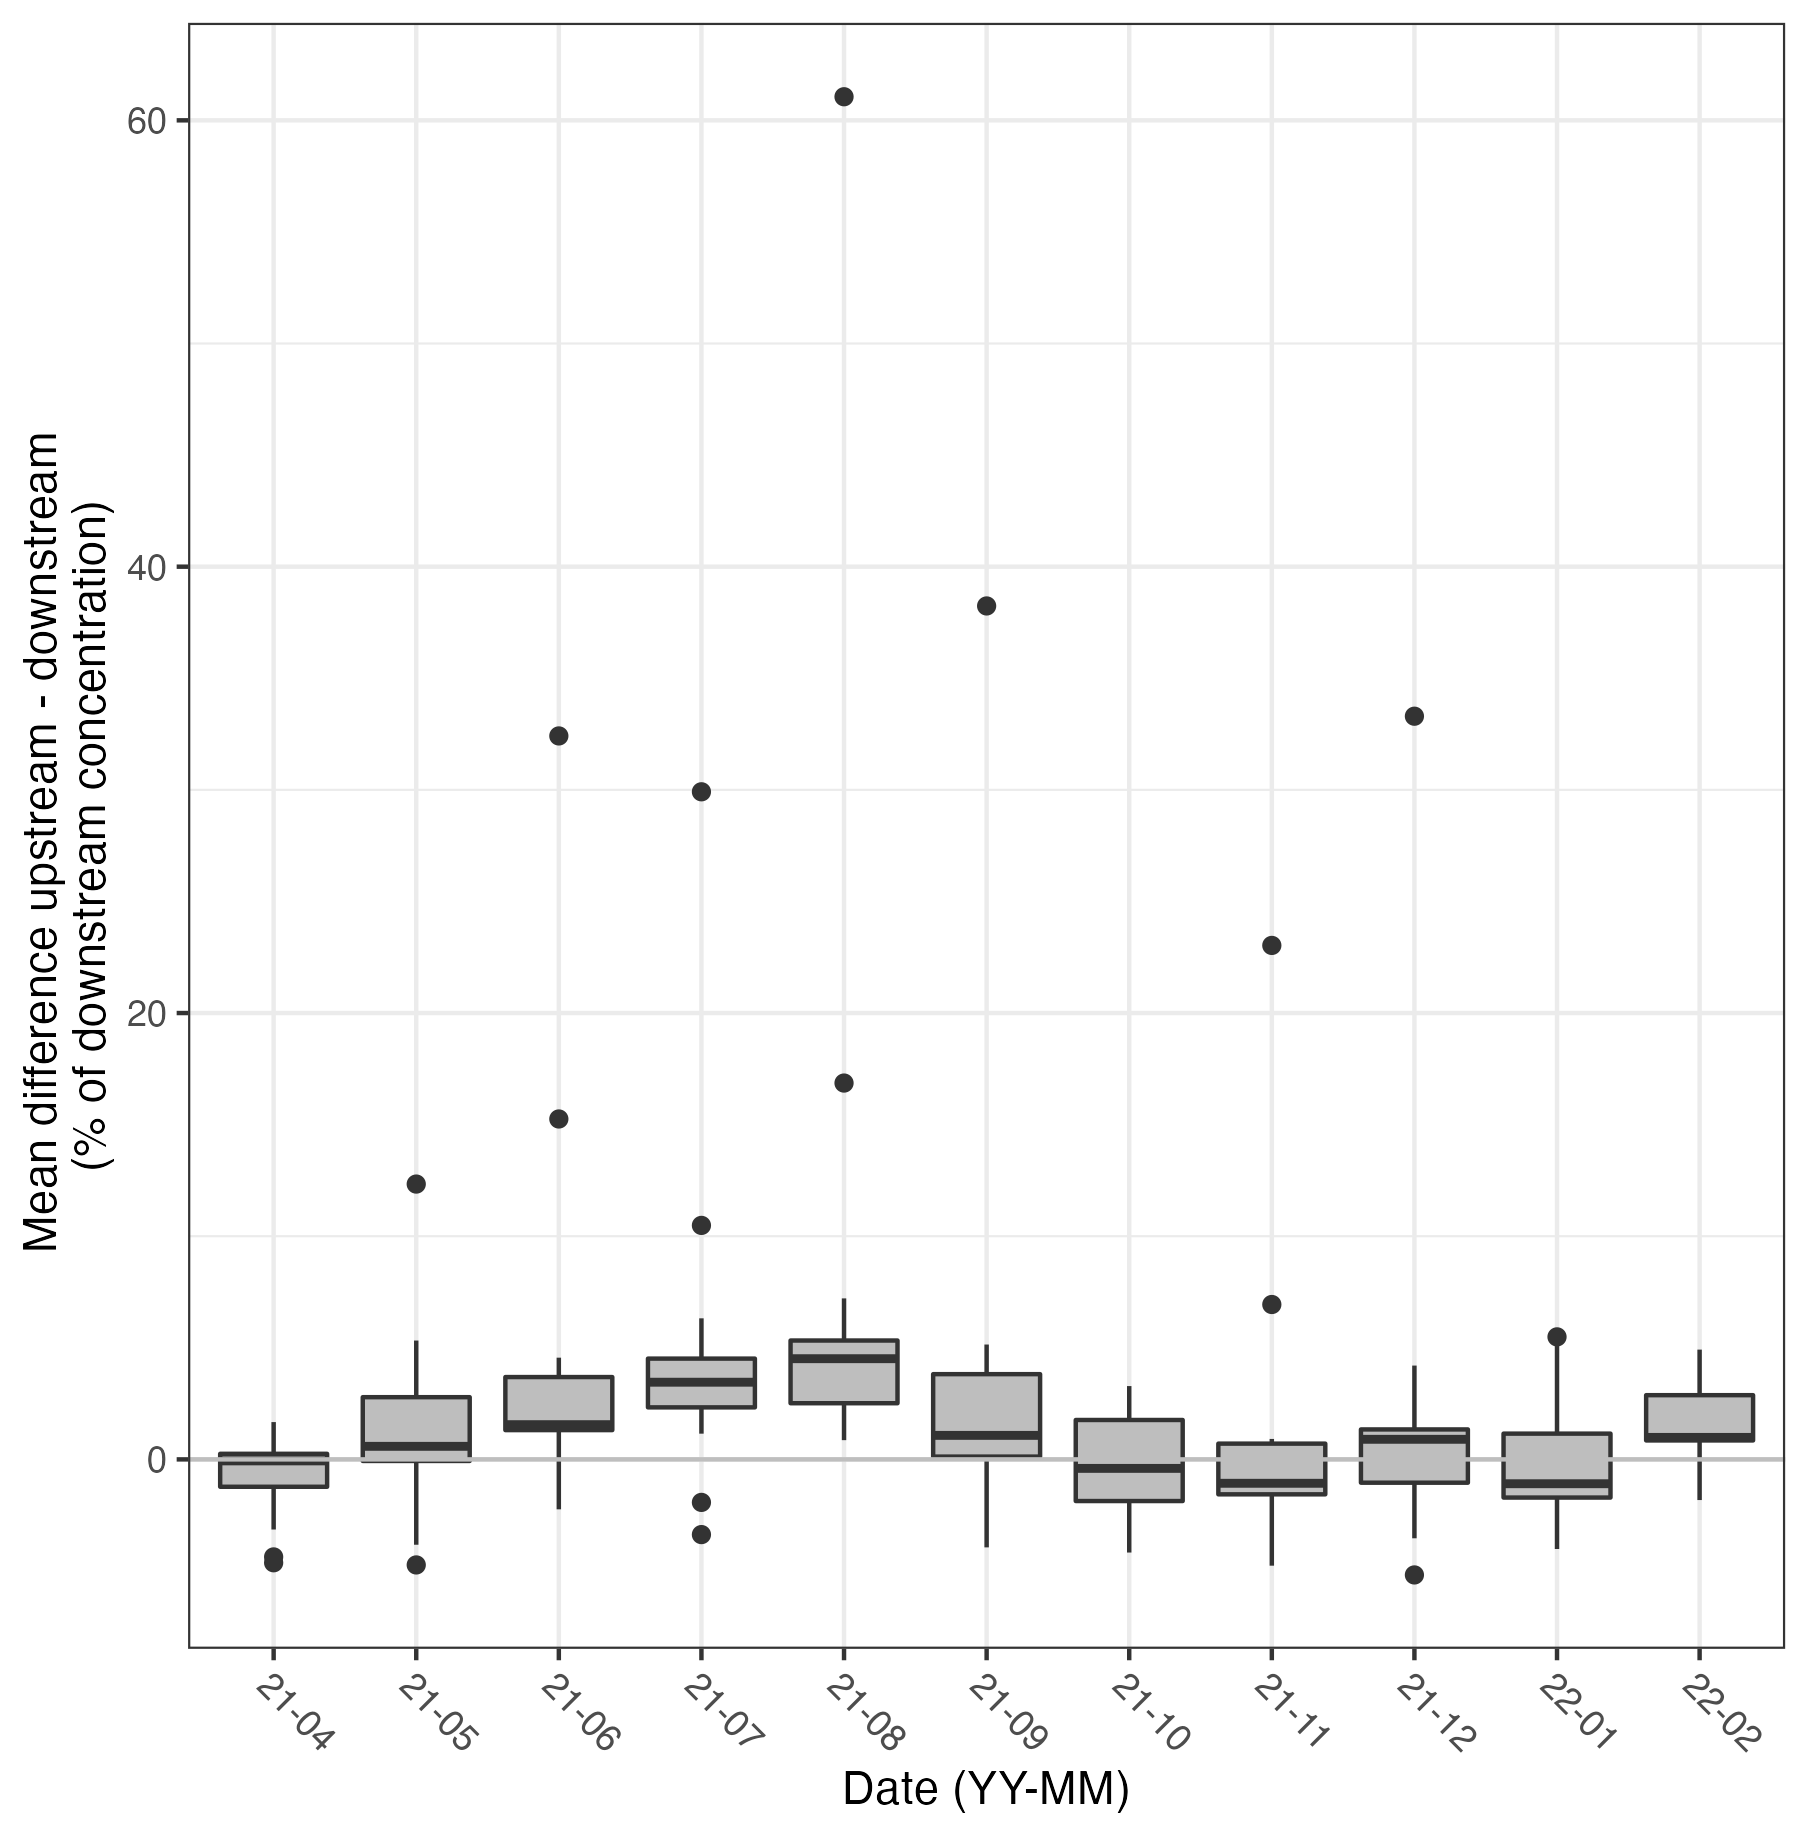
\includegraphics[width=0.6\textwidth,height=\textheight]{../Output/Figures/20221129_culvert_effect_flowcorrected.png}
\caption{The effect of culvert on salmonid abundance summed across all
species and creeks by time. The y-axis shows the difference between
upstream and downstream concentrations, normalized by downstream
concentration. The box boundaries correspond to the 25th and 75th
percentiles; the whiskers correspond to 1.5 times the interquartile
range.\label{fig:culverts}}
\end{figure}

\hypertarget{effects-of-culvert-removal}{%
\subsubsection{Effects of Culvert
Removal}\label{effects-of-culvert-removal}}

The effects of the culvert removal operation appear to have been
transient and fairly minor for the four salmonid species surveyed. After
the beginning of construction in September 2021 through the end of
sampling in February 2022, we see fluctuations in the percent changes of
salmonid DNA due to the culvert removal (Figure \ref{fig:construction}).
\emph{O. clarkii} is the least impacted species of the construction and
\emph{O. nerka} and \emph{O. mykiss} were the most impacted species,
likely due to their already low concentrations in the creek. For all
species, a very slight drop in concentration occurs in September and
October (ca. 5-20\% depending on the species), followed by an clear
increase in November (ca. 20-50\% depending on the species), and then a
stabilization of the concentration in December through February.

Of note, fish were exluded from Padden Creek on August 30th, 2021 in
preparation for the stream to be diverted on September 9th, 2021 and the
diversion was removed October 7th, 2021. Water sampling occurred on
September 10th, 2021, the day after the diversion, and on October 12,
2021, just 5 days after reconnecting the stream (Supplemental Table 1).

\begin{figure}
\centering
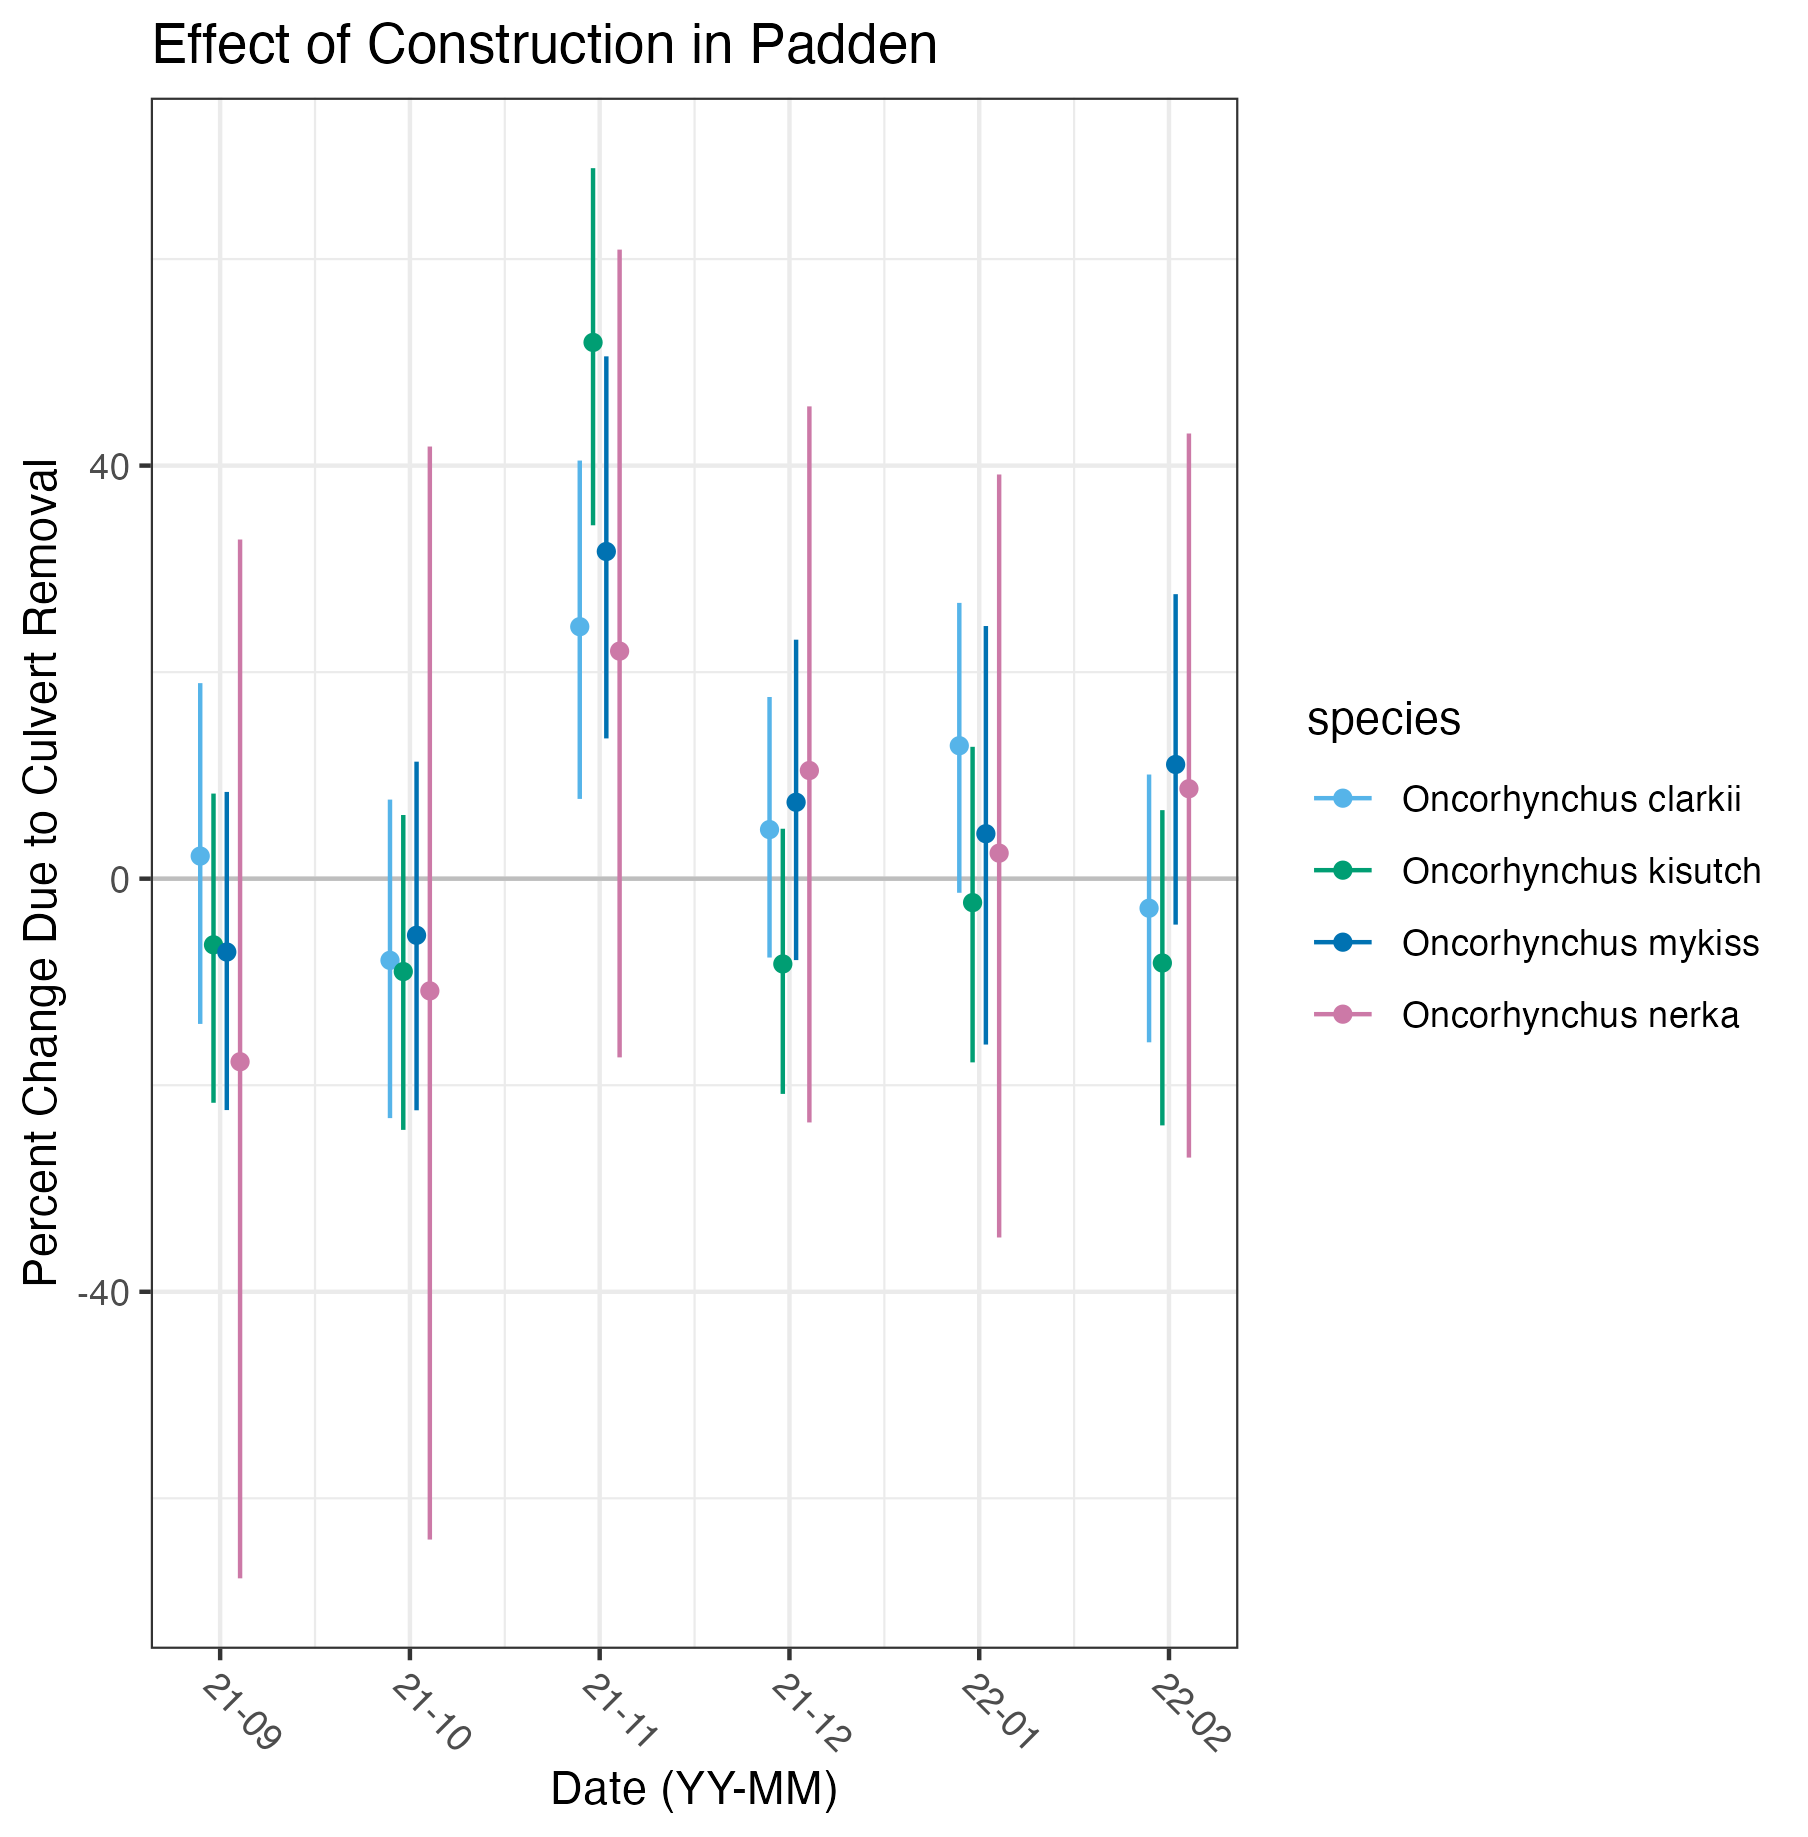
\includegraphics[width=0.6\textwidth,height=\textheight]{../Output/Figures/20221129_Construction_effect.png}
\caption{Effect of Construction on DNA Concentrations in Padden Creek.
Error bars show 95\% confidence intervals.\label{fig:construction}}
\end{figure}

\hypertarget{discussion}{%
\subsection{Discussion}\label{discussion}}

\hypertarget{environmental-dna-can-provide-quantitative-measurements-of-environmental-impacts}{%
\subsubsection{Environmental DNA can provide quantitative measurements
of environmental
impacts}\label{environmental-dna-can-provide-quantitative-measurements-of-environmental-impacts}}

A clear seasonal pattern occurred for all the salmonids detected in the
study. The time series model uses shared information across creeks to
include the change in eDNA concentrations due to time, whether a sample
was collected below or above a barrier (i.e., culvert), and whether or
not there was construction occurring. Thus, we could isolate the changes
in eDNA concentrations as a result of the intervention (i.e.,
construction) while accounting for the variance due to time and station
(i.e., season and culvert).

Furthermore, we can use just one qPCR assay in combination with
metabarcoding data to get information about many more species without
running n qPCR assays for n species detected in metabarcoding data
(which is also particularly helpful for species that don't have a
previously published assay). Metabarcoding data alone only gives
compositional data, which cannot be used in a time series to quantify
environmental impacts because there is no information about absolute
eDNA concentrations. However, by anchoring or grounding proportions
using a single qPCR assay, the proportional data can be turned into
quantitative data. The species for which to run the qPCR assay can be
determined after the metabarcoding is completed; the most commonly found
species with a robust qPCR assay should be used to glean the most
information.

This analysis also requires correcting metabarcoding data for different
species having different amplification efficiencies for a given primer
set and thermocycling conditions. For many years it has been
acknowledged that amplification bias occurs as demonstrated by the
disagreement between starting proportions of DNA before PCR with the
resulting proportions of sequencing reads (see Port et al. (2015);
Andruszkiewicz et al. (2017) and others for empirical data and Kelly et
al. (2019) for simulated data). Because PCR amplification is an
exponential process, even very slight differences in how well species
are amplified can result in large changes in sequencing reads (Shelton
et al., 2022). Here, we emphasize the importance of correcting
metabarcoding data for differences in amplification efficiencies when
using eDNA metabarcoding data for analysis that requires quantitative
data such as environmental impact assessments.

A few other studies have used eDNA to measure environmental impacts in
rivers and streams. Duda et al. (2021) used 11 species-specific qPCR
assays to document the distribution of resident and migratory fish after
a large dam removal (Elwah Dam in Port Angeles, Washington). No eDNA
sampling was conducted before the dam removal, but the study provided a
wealth of information about species returning after the dam removal.
Similarly, Muha et al. (2017) sampled three locations upstream and three
locations downstream before and after the removal of a weir that was
thought to be a barrier to salmonid migrations. The authors only sampled
once before and twice after the removal, spanning about a year, and used
eDNA metabarcoding to look at the presence/absence of species detected.
They found that in fact the before sample demonstrated that the weir was
not preventing fish passage (similar to the results found in this study)
and furthermore documented a slight increase in alpha diversity in the
first time point after the barrier removal and then a return to a
similar alpha diversity in the second time point after the removal
(similar results found in this study using eDNA concentrations rather
than diversity). Here, we used both eDNA metabarcoding and a single qPCR
assay on higher temporal resolution samples with control creeks to more
rigorously quantify both the effect of culverts and the impact of
construction on salmonids.

\hypertarget{not-all-culverts-are-barriers-to-salmonids}{%
\subsubsection{Not all culverts are barriers to
salmonids}\label{not-all-culverts-are-barriers-to-salmonids}}

By measuring DNA concentrations of salmonid species above and below
culverts on a small spatial scale, we were able to determine how much of
a barrier each culvert was (or was not) to fish passage. We found that
four of the five creeks sampled did not seem to be major barriers to
fish passage. The only creek that was determined to be a barrier to fish
passage was Barnes Creek, as we only found salmonid DNA in three months
of the twelve months of sampling, and those three months had very low
concentration of salmonid DNA relative to the other creeks.

Of the creeks where salmonid DNA was consistently found, Chuckanut Creek
had the largest discrepancies between DNA concentrations found below and
above the barrier at each time point. The culvert in Chuckanut Creek is
suspected to be a barrier to fish passage and the State of Washington's
Department of Transportation is planning to replace it in the near
future. The culverts at Portage Creek and Squalicum Creek were more
recently installed as compared to Padden, Chuckanut, and Barnes Creeks.
They also were not designated as blocking fish passage. Squalicum Creek
had the lowest difference between upstream and downstream concentrations
across all the surveyed creeks, which corresponds well with the
classification that the culvert does not block fish passage. Also,
Squalicum Creek is the only creek sampled that has baffles inside the
culvert of the five sampled, which should help fish passage.

Here, we demonstrate that collecting water samples for eDNA analysis
might help to prioritize restoration of culverts suspected to be
barriers to salmonids. Presently, the prioritization process conducted
by the Washington Department of Transportation is a protocol provided by
the Washington Department of Fish and Wildlife, which includes factors
such as the amount of habitat blocked by the barrier, the types of
species blocked by the barrier, and estimated cost of repair, among
other things (Fish and Wildlife, 2019). However, data on fish presence
upstream of barriers is rare and often not included in assessments.
Using eDNA as a proxy for fish presence could provide another important
type of data for project prioritization and increase efficiency in
making prioritization decisions.

Furthermore, the post-restoration monitoring efforts also focus
primarily on physical measurements (channel width, stream-bed material,
hydraulic drops, etc.) but surveys of fish are not required despite the
large costs associated with making culverts fish passable. Sampling
water for eDNA analysis could be done at the same time as the physical
measurements post-restoration by the same technicians conducting the
evaluation and provide valuable information on if the restoration
efforts did in fact allow for fish passage.

\hypertarget{salmonids-can-survive-a-bulldozer-in-a-creek}{%
\subsubsection{Salmonids can survive a bulldozer in a
creek}\label{salmonids-can-survive-a-bulldozer-in-a-creek}}

The intervention (i.e., construction) in Padden Creek occurred over
about two months and included the ``de-watering'' of the creek, removal
of the existing culvert, installation of the new culvert, and then the
``re-watering'' of the creek from late August 2021 to October 2021. The
impact of the construction itself on salmonid species demonstrates an
initial decrease in DNA concentrations in September and October,
followed by a large increase in DNA concentration in November, and then
a stabilization and return to nearly baseline concentrations from
December to February. This pattern remarkably demonstrates an expected
response to a large intervention. During the actual construction, we
found less eDNA from salmonids, but after the completion of the
installing a new culvert, concentrations increased and then returned to
baseline or near baseline, depending on the species.

The overall pattern of this effect was similar for the four species of
salmonids, but the species of which we found higher eDNA concentrations
seemed to have a dampened effect compared to the rarer species (i.e.,
\emph{O. clarkii} and \emph{O. kisutch} as compared to \emph{O. mykiss}
and \emph{O. nerka}). This also corresponds to species with different
life histories and behaviors, and it might be that our most commonly and
abundant species, \emph{O. clarkii}, was more robust to the intervention
because it has both migrating and non-migrating subspecies (see below).

\hypertarget{fish-ecology-and-expected-patterns}{%
\subsubsection{Fish ecology and expected
patterns}\label{fish-ecology-and-expected-patterns}}

Not all four salmonids are expected to be found in all five of the
creeks sampled. As documented by WA Department of Fish and Wildlife
SalmonScape (\url{http://apps.wdfw.wa.gov/salmonscape/map.html}), all
creeks contain cutthroat trout, steelhead trout, and coho salmon. Barnes
Creek is the only creek documented to have kokanee salmon. However,
local spawner surveys conducted by the City of Bellingham from 2015-2020
in Padden Creek document kokanee salmon as well as the other three
species and importantly, several unknown live and dead fish and redds
(nests dug by fish in gravel to deposit eggs).

The four salmonid species in this study have different ecologies and
behaviors that would impact when fish (and therefore eDNA
concentrations) occur in the creeks. For these four migratory salmonids,
the run timings vary for each species in the study area (Bellingham,
WA). Coastal cutthroat (\emph{O. clarkii}) are documented to run
throughout the entire year, whereas coho salmon (\emph{O. kisutch}) run
from September to December, kokanee salmon (\emph{O. nerka}) run from
October to December, and steelhead trout (\emph{O. mykiss}) run from
November to June.

Furthermore, three of the four species in this study have both migrating
and non-migrating subspecies that are not able to be distinguished
genetically. Cutthroat trout (\emph{O. clarkii}) encompasses both
non-migrating, resident trout in the creeks and coastal run cutthroat
that migrate into Padden Creek from Bellingham Bay. Similarly, \emph{O.
nerka} includes both anadromous sockeye salmon and non-migrating kokanee
salmon and \emph{O. mykiss} includes both anadromous steelhead trout and
non-migrating rainbow trout. Using eDNA, we cannot distinguish between
the migrating and non-migrating subspecies of \emph{O. clarkii},
\emph{O. nerka}, and \emph{O. mykiss}. Therefore, our eDNA
concentrations might reflect contributions from both migrating and
non-migrating individuals at any given time point in the dataset.

Despite the mix of migrating and non-migrating populations and various
run timings, our metabarcoding data demonstrates that in Padden Creek,
there was a clear signal of \emph{O. nerka} both upstream and downstream
only in November 2021-2022 (and only upstream in March 2021). This
signal corresponds well with the documented run timing of October to
December. In contrast, \emph{O. clarkii} and \emph{O. kisutch} were
found nearly year-round in Padden Creek. The persistent signal from
\emph{O. clarkii} could be explained by resident cutthroat trout.
However, \emph{O. kisutch} does not have a resident subspecies and the
run timing is only documented from September to December. This could
potentially be due to juveniles maturing and migrating in the creeks
after adults migrate during the run time up the creeks to spawn. Visual
surveys are conducted rarely and even if they were conducted, it might
be difficult to identify juveniles to species level. Though \emph{O.
kisutch} eDNA was found year round, the highest concentrations were
found near the expected run timing. Finally, though the lowest
concentrations on average, \emph{O. mykiss} was also found nearly
year-round in Padden Creek, which could be contributions from migrating
steelhead (November to June), juveniles maturing and migrating, or from
residential rainbow trout. Though the \emph{O. mykiss} signal is found
year-round, the highest concentrations do seem to correspond with the
steelhead run timing.

\hypertarget{decoupling-of-edna-from-fish}{%
\subsubsection{Decoupling of eDNA from
fish}\label{decoupling-of-edna-from-fish}}

By capturing residual eDNA from water samples, we are measuring a
different signal than counting how many fish are in the creek at each
time of sampling. We should not expect the eDNA concentration for each
salmonid to match the number of fish in the creek at the time of
sampling, especially as we often did not visually see any fish when we
took water samples. Shelton et al. (2019) provides a paired eDNA
sampling and seine netting analysis demonstrating that eDNA
concentrations provide a smoothed biological signal over space and time.
We acknowledge this smoothing effect and emphasize that in the context
of using eDNA for environmental impact assessments, it is preferable to
use a survey technique such as eDNA that represents a larger spatial and
temporal scale.

Many previous papers have commented on the ``ecology'' of eDNA and the
various processes that contribute to eDNA concentrations in
environmental samples (e.g., shedding rates, decay rates, transport).
For example, higher concentrations of eDNA could be the result of a
greater number (or biomass) of fish present, or increased shedding
rates, or decreased decay. Many review papers document the nuances of
interpreting eDNA data and we recommend reviewing them for a deeper
understanding (see Andruszkiewicz Allan et al. (2020) for a review on
shedding and decay rates and Harrison et al. (2019) for a review on
transport).

In this study, to assess the impact of a culvert on fish passage, we
compare eDNA concentrations upstream and downstream at the same time
point in a given creek. The distance between the upstream and downstream
sampling was minimal (\textasciitilde60-300 m, average distance of
\textasciitilde150 m). Therefore, we assume that the small differences
in spatial and temporal scale between sampling locations is minimal such
that the impacts of these various processes will affect the downstream
and upstream concentrations equally.

For assessing the impact of construction, we needed to account for
differences within the same creek over time (i.e., before and after
construction). Because the sampling occured over a whole year, transport
and persistence times may have varied. However, the time series model
uses information from the control creeks to understand seasonal trends
in eDNA concentrations without needing to link eDNA concentrations to
fish abundance. The impact of construction in Padden Creek can be
measured by comparing the meaured eDNA concentration during the time of
construction to the expected eDNA concentration in the absence of
construction by using information shared from the four other creeks that
are not undergoing construction. However, we did correct eDNA
concentrations {[}mass/volume{]} by discharge {[}volume/time{]} and use
a mass flow rate {[}mass/time{]} for the time series model (see below)
given the wide range of discharge over the course of the year.

\hypertarget{accounting-for-flow-with-edna-concentrations}{%
\subsubsection{Accounting for flow with eDNA
concentrations}\label{accounting-for-flow-with-edna-concentrations}}

Over the course of the year of sampling, water discharge varied from
very low to no flow in summer months to high flow in winter months. When
considering eDNA concentrations at a site, we need to account for the
large difference in water volume over the course of the time series. In
other words, given the same number of fish and a constant eDNA shedding
rate, we would expect to see higher concentrations of DNA in summer
months and lower concentrations in winter months due to dilution of eDNA
in higher water volumes just from the difference in flow. Other eDNA
time series datasets also correct for discharge to present eDNA data as
a mass flow rate {[}mass/time{]} (Thalinger et al., 2019; Tillotson et
al., 2018).

Though eDNA can move downstream with water flow, here, we were measuring
if culverts were barriers to fish moving upstream, as we were focused on
the impact of culverts on migratory salmon. In our case, we were
comparing if downstream stations had higher DNA concentrations than
upstream stations as a result of fish being unable to get upstream. This
is of course complicated as a result of non-migratory fish, which may be
up or downstream and not attempting to pass through the culverts.
However, the limited spatial scale between upstream and downstream is
such that we can assume the transport would affect upstream and
downstream locations in the same way. That is, in the upstream station,
some amount of eDNA is coming from upstream of that location into the
sampling station and leaving at the same time --- in the same way that
eDNA would be both entering and exiting the downstream station.
Therefore, the relative change between upstream and downstream stations
should be the same in terms of eDNA transport.

Other studies have documented the relative importance of eDNA transport.
Most notably, Tillotson et al. (2018) measured eDNA at four sites with
similar discharge rates to the creeks here and specifically addressed
spatial and temporal resolutions, finding that eDNA concentrations
reflect short time- (and therefore length-) scales by comparing peaks in
eDNA concentrations to counts of salmon and accumulation by measuring
both upstream and downstream sites. The authors found that the sampling
site furthest downstream did not accumulate eDNA and that two
tributaries feeding into a main channel were additive (Tillotson et al.,
2018). For more general models and empirical data documenting transport
distances in streams, see Wilcox et al. (2016), Jane et al. (2014),
Jerde et al. (2016), Shogren et al. (2016), and Civade et al. (2016).

Finally, it should be noted that Lake Padden, about 1.5 km upstream from
the sampling sites, was stocked with cutthroat trout in January 2021,
rainbow trout in April and May 2021, and kokanee salmon in May 2021.
Given that no sequencing reads in the metabarcoding data are found for
\emph{O. nerka} in May, the potential transport of eDNA downstream from
Lake Padden to the location of eDNA sampling is expected to be
negligible. Futhermore, Lake Padden is open for recreational fishing for
all of these species and managers have reported that most of the stocked
fish are caught soon after stocking. Given the transport distances
documented in the literature and flow rates in Lake Padden, we do not
expect the stocking in Lake Padden to affect eDNA concentrations at the
sampling locations.

\hypertarget{conclusion}{%
\subsection{Conclusion}\label{conclusion}}

It is notoriously difficult to quantify the environmental impact of
discrete human impacts on ecosystems and species. Surveying species and
communities by eDNA provides an opportunity for monitoring before,
during, and after impacts in a scaleable and cost-effective way. Here,
we demonstrate that monthly eDNA sampling before, during, and after an
intervention alongside control sites for one year can quantify the
environmental impact of replacing a road culvert. We also provide a
framework in which compositional metabarcoding data can be linked with
qPCR data to obtain quantitative estimates of eDNA concentrations of
many species. This provides a scaleable way to utilize the large amount
of information from metabarcoding data without needing a unique qPCR
assay for every species of interest. Environmental DNA is moving into
practice and this study demonstrates how eDNA can be broadly used for
environmental impact assessments for a wide range of species and
environments.

\hypertarget{references}{%
\subsection*{References}\label{references}}
\addcontentsline{toc}{subsection}{References}

\hypertarget{refs}{}
\begin{CSLReferences}{1}{0}
\leavevmode\vadjust pre{\hypertarget{ref-andruszkiewiczallan2020}{}}%
Andruszkiewicz Allan, E., Zhang, W.G., Lavery, A., Govindarajan, A.,
2020. Environmental DNA shedding and decay rates from diverse animal
forms and thermal regimes. Environmental DNA edn3.141.
\url{https://doi.org/10.1002/edn3.141}

\leavevmode\vadjust pre{\hypertarget{ref-andruszkiewicz2017}{}}%
Andruszkiewicz, E.A., Starks, H.A., Chavez, F.P., Sassoubre, L.M.,
Block, B.A., Boehm, A.B., 2017. Biomonitoring of marine vertebrates in
monterey bay using eDNA metabarcoding. PLOS ONE 12, e017634320.

\leavevmode\vadjust pre{\hypertarget{ref-benedetti-cecchi2001}{}}%
Benedetti-Cecchi, L., 2001. Beyond Baci: Optimization of Environmental
Sampling Designs Through Monitoring and Simulation. Ecological
Applications 11, 783--799.
https://doi.org/\url{https://doi.org/10.1890/1051-0761(2001)011\%5B0783:BBOOES\%5D2.0.CO;2}

\leavevmode\vadjust pre{\hypertarget{ref-buxton2021}{}}%
Buxton, A., Matechou, E., Griffin, J., Diana, A., Griffiths, R.A., 2021.
Optimising sampling and analysis protocols in environmental DNA studies.
Scientific Reports 11, 11637.
\url{https://doi.org/10.1038/s41598-021-91166-7}

\leavevmode\vadjust pre{\hypertarget{ref-callahan2016}{}}%
Callahan, B.J., McMurdie, P.J., Rosen, M.J., Han, A.W., Johnson, A.J.A.,
Holmes, S.P., 2016. DADA2: High resolution sample inference from
illumina amplicon data. Nature methods 13, 581--583.
\url{https://doi.org/10.1038/nmeth.3869}

\leavevmode\vadjust pre{\hypertarget{ref-camacho2009}{}}%
Camacho, C., Coulouris, G., Avagyan, V., Ma, N., Papadopoulos, J.,
Bealer, K., Madden, T.L., 2009. BLAST+: Architecture and applications.
BMC Bioinformatics 10, 4219.

\leavevmode\vadjust pre{\hypertarget{ref-civade2016}{}}%
Civade, R.l., Dejean, T., Valentini, A., Roset, N., Raymond, J.-C.,
Bonin, A., Taberlet, P., Pont, D., 2016. Spatial representativeness of
environmental DNA metabarcoding signal for fish biodiversity assessment
in a natural freshwater system. PLOS ONE 11, e015736619.

\leavevmode\vadjust pre{\hypertarget{ref-devargas2015}{}}%
De Vargas, C., Audie, S., Henry, N., Decelle, J., Mahe, F., Logares, R.,
Lara, E., Berney, C., Le Bescot, N., Probert, I., Carmichael, M.,
Poulain, J., Romac, S., Colin, S., Aury, J.-M., Bittner, L., Chaffron,
S., Dunthorn, M., Engelen, S., Flegontova, O., Guidi, L., Horak, A.,
Jaillon, O., Lima-Mendez, G., Lukes, J., Malviya, S., Morard, R., Mulot,
M., Scalco, E., Siano, R., Vincent, F., Zingone, A., Dimier, C.,
Picheral, M., Searson, S., Kandels-Lewis, S., coordinators, T.O.,
Acinas, S.G., Bork, P., Bowler, C., Gorsky, G., Grimsley, N., Hingamp,
P., Iudicone, D., Not, F., Ogata, H., Pesant, S., Raes, J., Sieracki,
M.E., Speich, S., Stemmann, L., Sunagawa, S., Weissenbach, J., Wincker,
P., Karsenti, E., 2015. Eukaryotic plankton diversity in the sunlit
ocean. Science 348, 112.

\leavevmode\vadjust pre{\hypertarget{ref-duda2021}{}}%
Duda, J.J., Hoy, M.S., Chase, D.M., Pess, G.R., Brenkman, S.J., McHenry,
M.M., Ostberg, C.O., 2021. Environmental DNA is an effective tool to
track recolonizing migratory fish following large-scale dam removal.
Environmental DNA 3, 121--141. \url{https://doi.org/10.1002/edn3.134}

\leavevmode\vadjust pre{\hypertarget{ref-washingtondepartmentoffishandwildlife2019}{}}%
Fish, W.D. of, Wildlife, 2019. Fish passage inventory, assessment, and
prioritization manual.

\leavevmode\vadjust pre{\hypertarget{ref-harrison2019}{}}%
Harrison, J.B., Sunday, J.M., Rogers, S.M., 2019. Predicting the fate of
eDNA in the environment and implications for studying biodiversity.
Proceedings of the Royal Society B: Biological Sciences 286, 20191409.
\url{https://doi.org/10.1098/rspb.2019.1409}

\leavevmode\vadjust pre{\hypertarget{ref-hinz2022}{}}%
Hinz, S., Coston-Guarini, J., Marnane, M., Guarini, J.-M., 2022.
Evaluating eDNA for Use within Marine Environmental Impact Assessments.
Journal of Marine Science and Engineering 10, 375.
\url{https://doi.org/10.3390/jmse10030375}

\leavevmode\vadjust pre{\hypertarget{ref-jane2014}{}}%
Jane, S.F., Wilcox, T.M., McKelvey, K.S., Young, M.K., Schwartz, M.K.,
Lowe, W.H., Letcher, B.H., Whiteley, A.R., 2014. Distance, flow and PCR
inhibition: eDNA dynamics in two headwater streams. Molecular Ecology
Resources 15, 216227.

\leavevmode\vadjust pre{\hypertarget{ref-jerde2016}{}}%
Jerde, C.L., Olds, B.P., Shogren, A.J., Andruszkiewicz, E.A., Mahon,
A.R., Bolster, D., Tank, J.L., 2016. Influence of stream bottom
substrate on retention and transport of vertebrate environmental DNA.
Environmental Science \& Technology 50, 87708779.

\leavevmode\vadjust pre{\hypertarget{ref-kelly2017}{}}%
Kelly, R.P., Closek, C.J., O'Donnell, J.L., Kralj, J.E., Shelton, A.O.,
Samhouri, J.F., 2017. Genetic and manual survey methods yield different
and complementary views of an ecosystem. Frontiers in Marine Science 3,
73511.

\leavevmode\vadjust pre{\hypertarget{ref-kelly2014}{}}%
Kelly, R.P., Port, J.A., Yamahara, K.M., Crowder, L.B., 2014. Using
environmental DNA to census marine fishes in a large mesocosm. PLOS ONE
9, e8617511.

\leavevmode\vadjust pre{\hypertarget{ref-kelly2019}{}}%
Kelly, R.P., Shelton, A.O., Gallego, R., 2019. Understanding PCR
Processes to Draw Meaningful Conclusions from Environmental DNA Studies.
Scientific Reports 9, 12133.
\url{https://doi.org/10.1038/s41598-019-48546-x}

\leavevmode\vadjust pre{\hypertarget{ref-klein2022}{}}%
Klein, S.G., Geraldi, N.R., Anton, A., Schmidt-Roach, S., Ziegler, M.,
Cziesielski, M.J., Martin, C., Rädecker, N., Frölicher, T.L., Mumby,
P.J., Pandolfi, J.M., Suggett, D.J., Voolstra, C.R., Aranda, M., Duarte,
Carlos.M., 2022. Projecting coral responses to intensifying marine
heatwaves under ocean acidification. Global Change Biology 28,
1753--1765. \url{https://doi.org/10.1111/gcb.15818}

\leavevmode\vadjust pre{\hypertarget{ref-leray2013}{}}%
Leray, M., Yang, J.Y., Meyer, C.P., Mills, S.C., Agudelo, N., Ranwez,
V., Boehm, J.T., Machida, R.J., 2013. A new versatile primer set
targeting a short fragment of the mitochondrial COI region for
metabarcoding metazoan diversity: Application for characterizing coral
reef fish gut contents. Frontiers in Zoology 10, 114.

\leavevmode\vadjust pre{\hypertarget{ref-maasri2022}{}}%
Maasri, A., Jähnig, S.C., Adamescu, M.C., Adrian, R., Baigun, C., Baird,
D.J., Batista-Morales, A., Bonada, N., Brown, L.E., Cai, Q.,
Campos-Silva, J.V., Clausnitzer, V., Contreras-MacBeath, T., Cooke,
S.J., Datry, T., Delacámara, G., De Meester, L., Dijkstra, K.-D.B., Do,
V.T., Domisch, S., Dudgeon, D., Erös, T., Freitag, H., Freyhof, J.,
Friedrich, J., Friedrichs-Manthey, M., Geist, J., Gessner, M.O.,
Goethals, P., Gollock, M., Gordon, C., Grossart, H.-P., Gulemvuga, G.,
Gutiérrez-Fonseca, P.E., Haase, P., Hering, D., Hahn, H.J., Hawkins,
C.P., He, F., Heino, J., Hermoso, V., Hogan, Z., Hölker, F., Jeschke,
J.M., Jiang, M., Johnson, R.K., Kalinkat, G., Karimov, B.K., Kasangaki,
A., Kimirei, I.A., Kohlmann, B., Kuemmerlen, M., Kuiper, J.J., Kupilas,
B., Langhans, S.D., Lansdown, R., Leese, F., Magbanua, F.S., Matsuzaki,
S.S., Monaghan, M.T., Mumladze, L., Muzon, J., Mvogo Ndongo, P.A.,
Nejstgaard, J.C., Nikitina, O., Ochs, C., Odume, O.N., Opperman, J.J.,
Patricio, H., Pauls, S.U., Raghavan, R., Ramírez, A., Rashni, B.,
Ross-Gillespie, V., Samways, M.J., Schäfer, R.B., Schmidt-Kloiber, A.,
Seehausen, O., Shah, D.N., Sharma, S., Soininen, J., Sommerwerk, N.,
Stockwell, J.D., Suhling, F., Tachamo Shah, R.D., Tharme, R.E., Thorp,
J.H., Tickner, D., Tockner, K., Tonkin, J.D., Valle, M., Vitule, J.,
Volk, M., Wang, D., Wolter, C., Worischka, S., 2022. A global agenda for
advancing freshwater biodiversity research. Ecology Letters 25,
255--263. \url{https://doi.org/10.1111/ele.13931}

\leavevmode\vadjust pre{\hypertarget{ref-martin2012}{}}%
Martin, C.J.B., Allen, B.J., Lowe, C.G., 2012. Environmental impact
assessment: Detecting changes in fish community structure in response to
disturbance with an asymmetric multivariate BACI sampling design.
Bulletin, Southern California Academy of Sciences 111, 119--131.
\url{https://doi.org/10.3160/0038-3872-111.2.119}

\leavevmode\vadjust pre{\hypertarget{ref-martin2011}{}}%
Martin, M., 2011. Cutadapt removes adapter sequences from
high-throughput sequencing reads. EMBnet.journal 17, 10.
\url{https://doi.org/10.14806/ej.17.1.200}

\leavevmode\vadjust pre{\hypertarget{ref-martinez2013}{}}%
Martinez, R., 2013. United states v. washington.

\leavevmode\vadjust pre{\hypertarget{ref-mccall2014}{}}%
McCall, M.N., McMurray, H.R., Land, H., Almudevar, A., 2014. On
non-detects in qPCR data. Bioinformatics 30, 2310--2316.
\url{https://doi.org/10.1093/bioinformatics/btu239}

\leavevmode\vadjust pre{\hypertarget{ref-mclaren2019}{}}%
McLaren, M.R., Willis, A.D., Callahan, B.J., 2019. Consistent and
correctable bias in metagenomic sequencing experiments. eLife 8, e46923.
\url{https://doi.org/10.7554/eLife.46923}

\leavevmode\vadjust pre{\hypertarget{ref-morgan2012}{}}%
Morgan, R.K., 2012. Environmental impact assessment: The state of the
art. Impact Assessment and Project Appraisal 30, 5--14.
\url{https://doi.org/10.1080/14615517.2012.661557}

\leavevmode\vadjust pre{\hypertarget{ref-moss2022}{}}%
Moss, W.E., Harper, L.R., Davis, M.A., Goldberg, C.S., Smith, M.M.,
Johnson, P.T.J., 2022. Navigating the trade-offs between environmental
DNA and conventional field surveys for improved amphibian monitoring.
Ecosphere 13, e3941. \url{https://doi.org/10.1002/ecs2.3941}

\leavevmode\vadjust pre{\hypertarget{ref-muha2017}{}}%
Muha, T.P., Rodríguez-Rey, M., Rolla, M., Tricarico, E., 2017. Using
environmental DNA to improve species distribution models for freshwater
invaders. Frontiers in Ecology and Evolution 5, 143957.

\leavevmode\vadjust pre{\hypertarget{ref-ogram1987}{}}%
Ogram, A., Sayler, G., Barkay, T., 1987. The extraction and purification
of microbial DNA from sediments. Journal of Microbiological Methods 7,
5766.

\leavevmode\vadjust pre{\hypertarget{ref-port2015}{}}%
Port, J.A., O'Donnell, J.L., Romero-Maraccini, O.C., Leary, P.R.,
Litvin, S.Y., Nickols, K.J., Yamahara, K.M., Kelly, R.P., 2015.
Assessing vertebrate biodiversity in a kelp forest ecosystem using
environmental DNA. Molecular Ecology 25, 527541.

\leavevmode\vadjust pre{\hypertarget{ref-rcoreteam2017}{}}%
R Core Team, 2017. R: A language and environment for statistical
computing. R Foundation for Statistical Computing.

\leavevmode\vadjust pre{\hypertarget{ref-rondon2000}{}}%
Rondon, M.R., August, P.R., Bettermann, A.D., Brady, S.F., Grossman,
T.H., Liles, M.R., Loiacono, K.A., Lynch, B.A., MacNeil, I.A., Minor,
C., Tiong, C.L., Gilman, M., Osburne, M.S., Clardy, J., Handelsman, J.,
Goodman, R.M., 2000. Cloning the soil metagenome: a strategy for
accessing the genetic and functional diversity of uncultured
microorganisms. Applied and Environmental Microbiology 66, 2541--2547.
\url{https://doi.org/10.1128/AEM.66.6.2541-2547.2000}

\leavevmode\vadjust pre{\hypertarget{ref-rubin2017}{}}%
Rubin, Z., Kondolf, G.M., Rios-Touma, B., 2017. Evaluating Stream
Restoration Projects: What Do We Learn from Monitoring? Water 9, 174.
\url{https://doi.org/10.3390/w9030174}

\leavevmode\vadjust pre{\hypertarget{ref-ruppert2019}{}}%
Ruppert, K.M., Kline, R.J., Rahman, M.S., 2019. Past, present, and
future perspectives of environmental DNA (eDNA) metabarcoding: A
systematic review in methods, monitoring, and applications of global
eDNA. Global Ecology and Conservation 17, e00547.
\url{https://doi.org/10.1016/j.gecco.2019.e00547}

\leavevmode\vadjust pre{\hypertarget{ref-seymour2021}{}}%
Seymour, M., Edwards, F.K., Cosby, B.J., Bista, I., Scarlett, P.M.,
Brailsford, F.L., Glanville, H.C., Bruyn, M. de, Carvalho, G.R., Creer,
S., 2021. Environmental DNA provides higher resolution assessment of
riverine biodiversity and ecosystem function via spatio-temporal
nestedness and turnover partitioning. Communications Biology 4, 1--12.
\url{https://doi.org/10.1038/s42003-021-02031-2}

\leavevmode\vadjust pre{\hypertarget{ref-shelton}{}}%
Shelton, A.O., Gold, Z.J., Jensen, A.J., D'Agnese, E., Andruszkiewicz
Allan, E., Van Cise, A., Gallego, R., Ramón-Laca, A., Garber-Yonts, M.,
Parsons, K., Kelly, R.P., 2022. Toward quantitative metabarcoding.
Ecology n/a, e3906. \url{https://doi.org/10.1002/ecy.3906}

\leavevmode\vadjust pre{\hypertarget{ref-shelton2019}{}}%
Shelton, A.O., Kelly, R.P., O'Donnell, J.L., Park, L., Schwenke, P.,
Greene, C., Henderson, R.A., Beamer, E.M., 2019. Environmental DNA
provides quantitative estimates of a threatened salmon species.
Biological Conservation 237, 383--391.
\url{https://doi.org/10.1016/j.biocon.2019.07.003}

\leavevmode\vadjust pre{\hypertarget{ref-shelton2016}{}}%
Shelton, A.O., O'Donnell, J.L., Samhouri, J.F., Lowell, N.C., Williams,
G.D., Kelly, R.P., 2016. A framework for inferring biological
communities from environmental DNA 115.

\leavevmode\vadjust pre{\hypertarget{ref-shogren2016}{}}%
Shogren, A.J., Tank, J.L., Andruszkiewicz, E.A., Olds, B.P., Jerde,
C.L., Bolster, D., 2016. Modelling the transport of environmental DNA
through a porous substrate using continuous flow-through column
experiments. Journal of The Royal Society Interface 13, 2016029011.

\leavevmode\vadjust pre{\hypertarget{ref-standevelopmentteam2022}{}}%
Stan Development Team, 2022. \href{https://mc-stan.org/}{RStan: The r
interface to stan.}

\leavevmode\vadjust pre{\hypertarget{ref-stat2017}{}}%
Stat, M., Huggett, M.J., Bernasconi, R., DiBattista, J.D., Berry, T.E.,
Newman, S.J., Harvey, E.S., Bunce, M., 2017. Ecosystem biomonitoring
with eDNA: Metabarcoding across the tree of life in a tropical marine
environment. Scientific Reports 111.

\leavevmode\vadjust pre{\hypertarget{ref-taberlet2012}{}}%
Taberlet, P., Coissac, E., Hajibabaei, M., Rieseberg, L.H., 2012.
Environmental DNA. Molecular Ecology 21, 17891793.

\leavevmode\vadjust pre{\hypertarget{ref-thalinger2019}{}}%
Thalinger, B., Wolf, E., Traugott, M., Wanzenböck, J., 2019. Monitoring
spawning migrations of potamodromous fish species via eDNA. Scientific
Reports 9, 15388. \url{https://doi.org/10.1038/s41598-019-51398-0}

\leavevmode\vadjust pre{\hypertarget{ref-thomas2018}{}}%
Thomas, A.C., Howard, J., Nguyen, P.L., Seimon, T.A., Goldberg, C.S.,
2018. ANDe {\texttrademark}: A fully integrated environmental DNA
sampling system. Methods in Ecology and Evolution 9, 13791385.

\leavevmode\vadjust pre{\hypertarget{ref-thomas2019}{}}%
Thomas, A.C., Nguyen, P.L., Howard, J., Goldberg, C.S., 2019. A
self-preserving, partially biodegradable eDNA filter. Methods in Ecology
and Evolution 10, 1136--1141.
\url{https://doi.org/10.1111/2041-210X.13212}

\leavevmode\vadjust pre{\hypertarget{ref-thomsen2015}{}}%
Thomsen, P.F., Willerslev, E., 2015. Environmental DNA: An emerging tool
in conservation for monitoring past and present biodiversity. Biological
Conservation 183, 418.

\leavevmode\vadjust pre{\hypertarget{ref-tillotson2018}{}}%
Tillotson, M.D., Kelly, R.P., Duda, J.J., Hoy, M., Kralj, J., Quinn,
T.P., 2018. Concentrations of environmental DNA (eDNA) reflect spawning
salmon abundance at fine spatial and temporal scales. Biological
Conservation 220, 111.

\leavevmode\vadjust pre{\hypertarget{ref-turnbaugh2007}{}}%
Turnbaugh, P.J., Ley, R.E., Hamady, M., Fraser-Liggett, C.M., Knight,
R., Gordon, J.I., 2007. The Human Microbiome Project. Nature 449,
804--810. \url{https://doi.org/10.1038/nature06244}

\leavevmode\vadjust pre{\hypertarget{ref-u.s.geologicalsurvey1994}{}}%
U. S. Geological Survey, 1994. USGS water data for the nation.
\url{https://doi.org/10.5066/F7P55KJN}

\leavevmode\vadjust pre{\hypertarget{ref-underwood1994}{}}%
Underwood, A.J., 1994. On Beyond BACI: Sampling Designs that Might
Reliably Detect Environmental Disturbances. Ecological Applications 4,
3--15. https://doi.org/\url{https://doi.org/10.2307/1942110}

\leavevmode\vadjust pre{\hypertarget{ref-underwood1992}{}}%
Underwood, A.J., 1992. Beyond BACI: the detection of environmental
impacts on populations in the real, but variable, world. Journal of
Experimental Marine Biology and Ecology 161, 145--178.
\url{https://doi.org/10.1016/0022-0981(92)90094-Q}

\leavevmode\vadjust pre{\hypertarget{ref-valentini2016}{}}%
Valentini, A., Taberlet, P., Miaud, C., Civade, R.l., Herder, J.E.,
Thomsen, P.F., Bellemain, E., Besnard, A., Coissac, E., Boyer, F.,
Gaboriaud, C., Jean, P., Poulet, N., Roset, N., Copp, G.H., Geniez, P.,
Pont, D., Argillier, C., Baudoin, J.-M., Peroux, T., Crivelli, A.J.,
Olivier, A., Acqueberge, M., Le Brun, M., Moller, P.R., Willerslev, E.,
Dejean, T., 2016. Next-generation monitoring of aquatic biodiversity
using environmental DNA metabarcoding. Molecular Ecology 25, 929942.

\leavevmode\vadjust pre{\hypertarget{ref-wilcox2016}{}}%
Wilcox, T.M., McKelvey, K.S., Young, M.K., Sepulveda, A.J., Shepard,
B.B., Jane, S.F., Whiteley, A.R., Lowe, W.H., Schwartz, M.K., 2016.
Understanding environmental DNA detection probabilities: A case study
using a stream-dwelling char salvelinus fontinalis. Biological
Conservation 194, 209216.

\leavevmode\vadjust pre{\hypertarget{ref-wilkinson2018}{}}%
Wilkinson, S.P., Davy, S.K., Bunce, M., Stat, M., 2018. Taxonomic
identification of environmental DNA with informatic sequence
classification trees.
\url{https://doi.org/10.7287/peerj.preprints.26812v1}

\end{CSLReferences}

\end{document}
